%=====================================================================%
% DOCUMENT DEFINITION
%=====================================================================%


\documentclass[12pt]{article}

\usepackage[english]{babel}

\usepackage{subcaption}

\usepackage{gensymb}

\usepackage{setspace}
\onehalfspacing

\usepackage[
    a4paper,
    top=2cm,
    bottom=2cm,
    left=2cm,
    right=2cm,
    marginparwidth=1.75cm
]{geometry}

\usepackage[skip=8pt plus1pt, indent=20pt]{parskip}

% inserting images
\usepackage{graphicx}
\usepackage{float}
\graphicspath{{images/}}

% references
\usepackage{csquotes}
\usepackage[
    backend=biber,
    style=numeric-comp,
    sorting=none
]{biblatex}
\addbibresource{references.bib}


% math
\usepackage{amsmath}
\usepackage{empheq}

% tables
\usepackage{booktabs}

% color
\usepackage{xcolor}

% dummy text
\usepackage{lipsum}


%=====================================================================%
% DOCUMENT
%=====================================================================%
\setlength{\parindent}{0pt} 


\begin{document}

%=====================================================================%
% TITLE PAGE
%=====================================================================%

\begin{titlepage}

\centering
\singlespacing

% ------------------------------------------------
% UNIVERSITY LOGO
% ------------------------------------------------

\includegraphics[width=0.70\textwidth]{bmelogo.png}

\vspace{0.4cm}

{\Large\bfseries
Budapest University of Technology and Economics\par}

\vspace{0.15cm}

{\Large Faculty of Natural Sciences\par}

% ------------------------------------------------
% TITLE
% ------------------------------------------------

\vspace{3.3cm}

{\LARGE\bfseries
M3 - Study of Comparators \\
\par}

\vspace{0.3cm}

{\Large Lab report\par}

% ------------------------------------------------
% DATE
% ------------------------------------------------

\vspace{2.6cm}

{\Large 04/11/2026\par}

% ------------------------------------------------
% LAB RESPONSIBLE
% ------------------------------------------------

\vspace{2.5cm}

{\Large
\underline{Lab responsible}\\[-0.05cm]
\textbf{Viktor Farkas}
\par}

% ------------------------------------------------
% STUDENTS
% ------------------------------------------------

\vfill

\begin{minipage}[t]{0.47\textwidth}
    \centering

    {\Large {Student}\par}

    \vspace{0.1cm}

    {\bfseries
    Abigél ORTUTAY (UGHRKC)\par}
     {\normalsize
    Physics-engineering BSc 3rd year\par}
    {\normalsize
    abico.ortutay@gmail.com}
    
\end{minipage}
\hfill
\begin{minipage}[t]{0.47\textwidth}
    \centering

    {\Large {Student}\par}
   

    \vspace{0.1cm}

    {\bfseries
    Hanna ERTL (SPH4U7)\par}
    {\normalsize
    Physics-engineering BSc 3rd year\par}
    {\normalsize
    hannavedaertl@gmail.com}
    
    
\end{minipage}

\vspace{1.3cm}

\end{titlepage}


%=====================================================================%
% REPORT STARTS HERE
%=====================================================================%
\begin{abstract}
    \noindent This laboratory experiment explored four voltage switching circuits: a simple operational amplifier comparator, an operational amplifier Schmitt trigger, a relaxation oscillator, and a two-transistor Schmitt trigger. Measurements showed that the basic comparator was limited by output saturation (-3.06 V and 4.47 V), the op-amp Schmitt trigger created a 0.50 V hysteresis band to prevent noise issues, and the lower slew rate $\mu$A741 op-amp distorted the oscillator signals compared to the faster TL071 op-amp. Finally, the transistor Schmitt trigger had switching thresholds at 1.25 V and 0.80 V to yield a 0.45 V hysteresis, showing strong overall agreement between our practical measurements and theoretical calculations.
\end{abstract}

\section{Theoretical introduction}
In this laboratory exercise we used two operational amplifiers - high speed 
TL071CP (slew rate $SR \approx 13\text{--}20\text{ V}/\mu\text{s}$) and the 
general purpose bipolar $\mu$A741CN (slew rate $SR \approx 0.5\text{ V}/\mu\text{s}$) 
— as well as BC182 NPN bipolar junction transistors for discrete logic switching.
The theoretical background of the four configurations used during this laboratory 
exercise are the following:\\\\
A basic op-amp comparator evaluates two input voltages and switches its output to 
either supply rail depending on which input is larger. The reference switching threshold U1 
at the non-inverting terminal is set by a passive voltage divider given by the equation: 
\begin{center} $U_1 = U_+ \cdot \frac{R_2}{R_1 + R_2}$ \end{center}
This results in the output voltage switching states whenever the inverting input voltage 
U2 crosses this threshold. This configuration is sensitive to input noise however, 
as the switching threshold is a distinct value and allows no "wiggle room" when switching states.\\\\
As a solution adding a feedback resistor R3 introduces positive feedback, establishing a noise-rejecting hysteresis band so small fluctuations do not cause unwanted output oscillations. The threshold voltage U1 dynamically shifts based on the current output state:
\begin{center} $U_1 = \frac{U_+}{1 + \frac{R_1}{R_2} + \frac{R_1}{R_3}} + \frac{U_{\text{out}}}{1 + \frac{R_3}{R_2} + \frac{R_3}{R_1}}$ \end{center}
which creates distinct upper ($U_{1+}$) and lower ($U_{1-}$) switching levels.\\\\
Combining positive feedback with an RC timing network allows the operational amplifier to generate continuous square and triangular waveforms without needing an external input signal. The capacitor repeatedly charges and discharges through R1 between the switching thresholds, yielding an oscillation period T and frequency f: 
\begin{center} $T = 2 \cdot R_1 \cdot C \cdot \ln\left(1 + \frac{2 R_2}{R_3}\right) \quad \text{and} \quad f = \frac{1}{T}$ \end{center}
\vspace{0.3cm}
A discrete Schmitt trigger uses two NPN transistors (T1, T2) sharing a common emitter resistor $R_E$ to achieve positive feedback and hysteresis. The switching thresholds occur when the base input voltage overcomes the shared emitter voltage plus the internal base-emitter diode turn-on drop represented by the equations: 
\begin{center} $U_{\text{in}} = U_E + U_{BE1} \quad \text{where} \quad U_E \approx \frac{U_{supp} - U_{CE,\text{sat}}}{R_C + R_E} \cdot R_E$ \end{center}
Because the active collector resistor changes depending on whether T1 or T2 is conducting, the shared emitter voltage $U_E$ shifts between two levels, establishing the upper and lower switching thresholds.

\section{Measurement tools}
For this measurement, we used the following list of tools:
\begin{itemize}
\item ST $\mu$A741CN operational amplifier
\item TI TL071CP operational amplifier
\item OK Industries Inc. CM-140 L breadboard
\item Resistors: 22 k$\Omega$ (1 piece), 10 k$\Omega$ (2 pieces), 100 k$\Omega$ (1 piece),  1 k$\Omega$ (1 piece)
\item Jumping wires (6 pieces)
\item Crocodile clips (6 pieces)
\item Banana plugs (6 pieces)
\item Capacitor: 6.8 nF (1 piece)
\item HM8040-2 HAMEG Triple power supply
\item HM 8011-3 HAMEG Digital multimeter
\item SIGLENT SDS 1072CML Digital storage oscilloscope
\item Handheld multimeter
\end{itemize}

\newpage \section{Measurement setup}

\pagebreak\section{Measurements}

\subsection{Switching voltage of the comparator with an operational\\ amplifier}

For the first measurement, we had the ciruit setup as seen on figure 1 
and described in the Measurement Setup section above.

\begin{figure}[H]
    \centering
    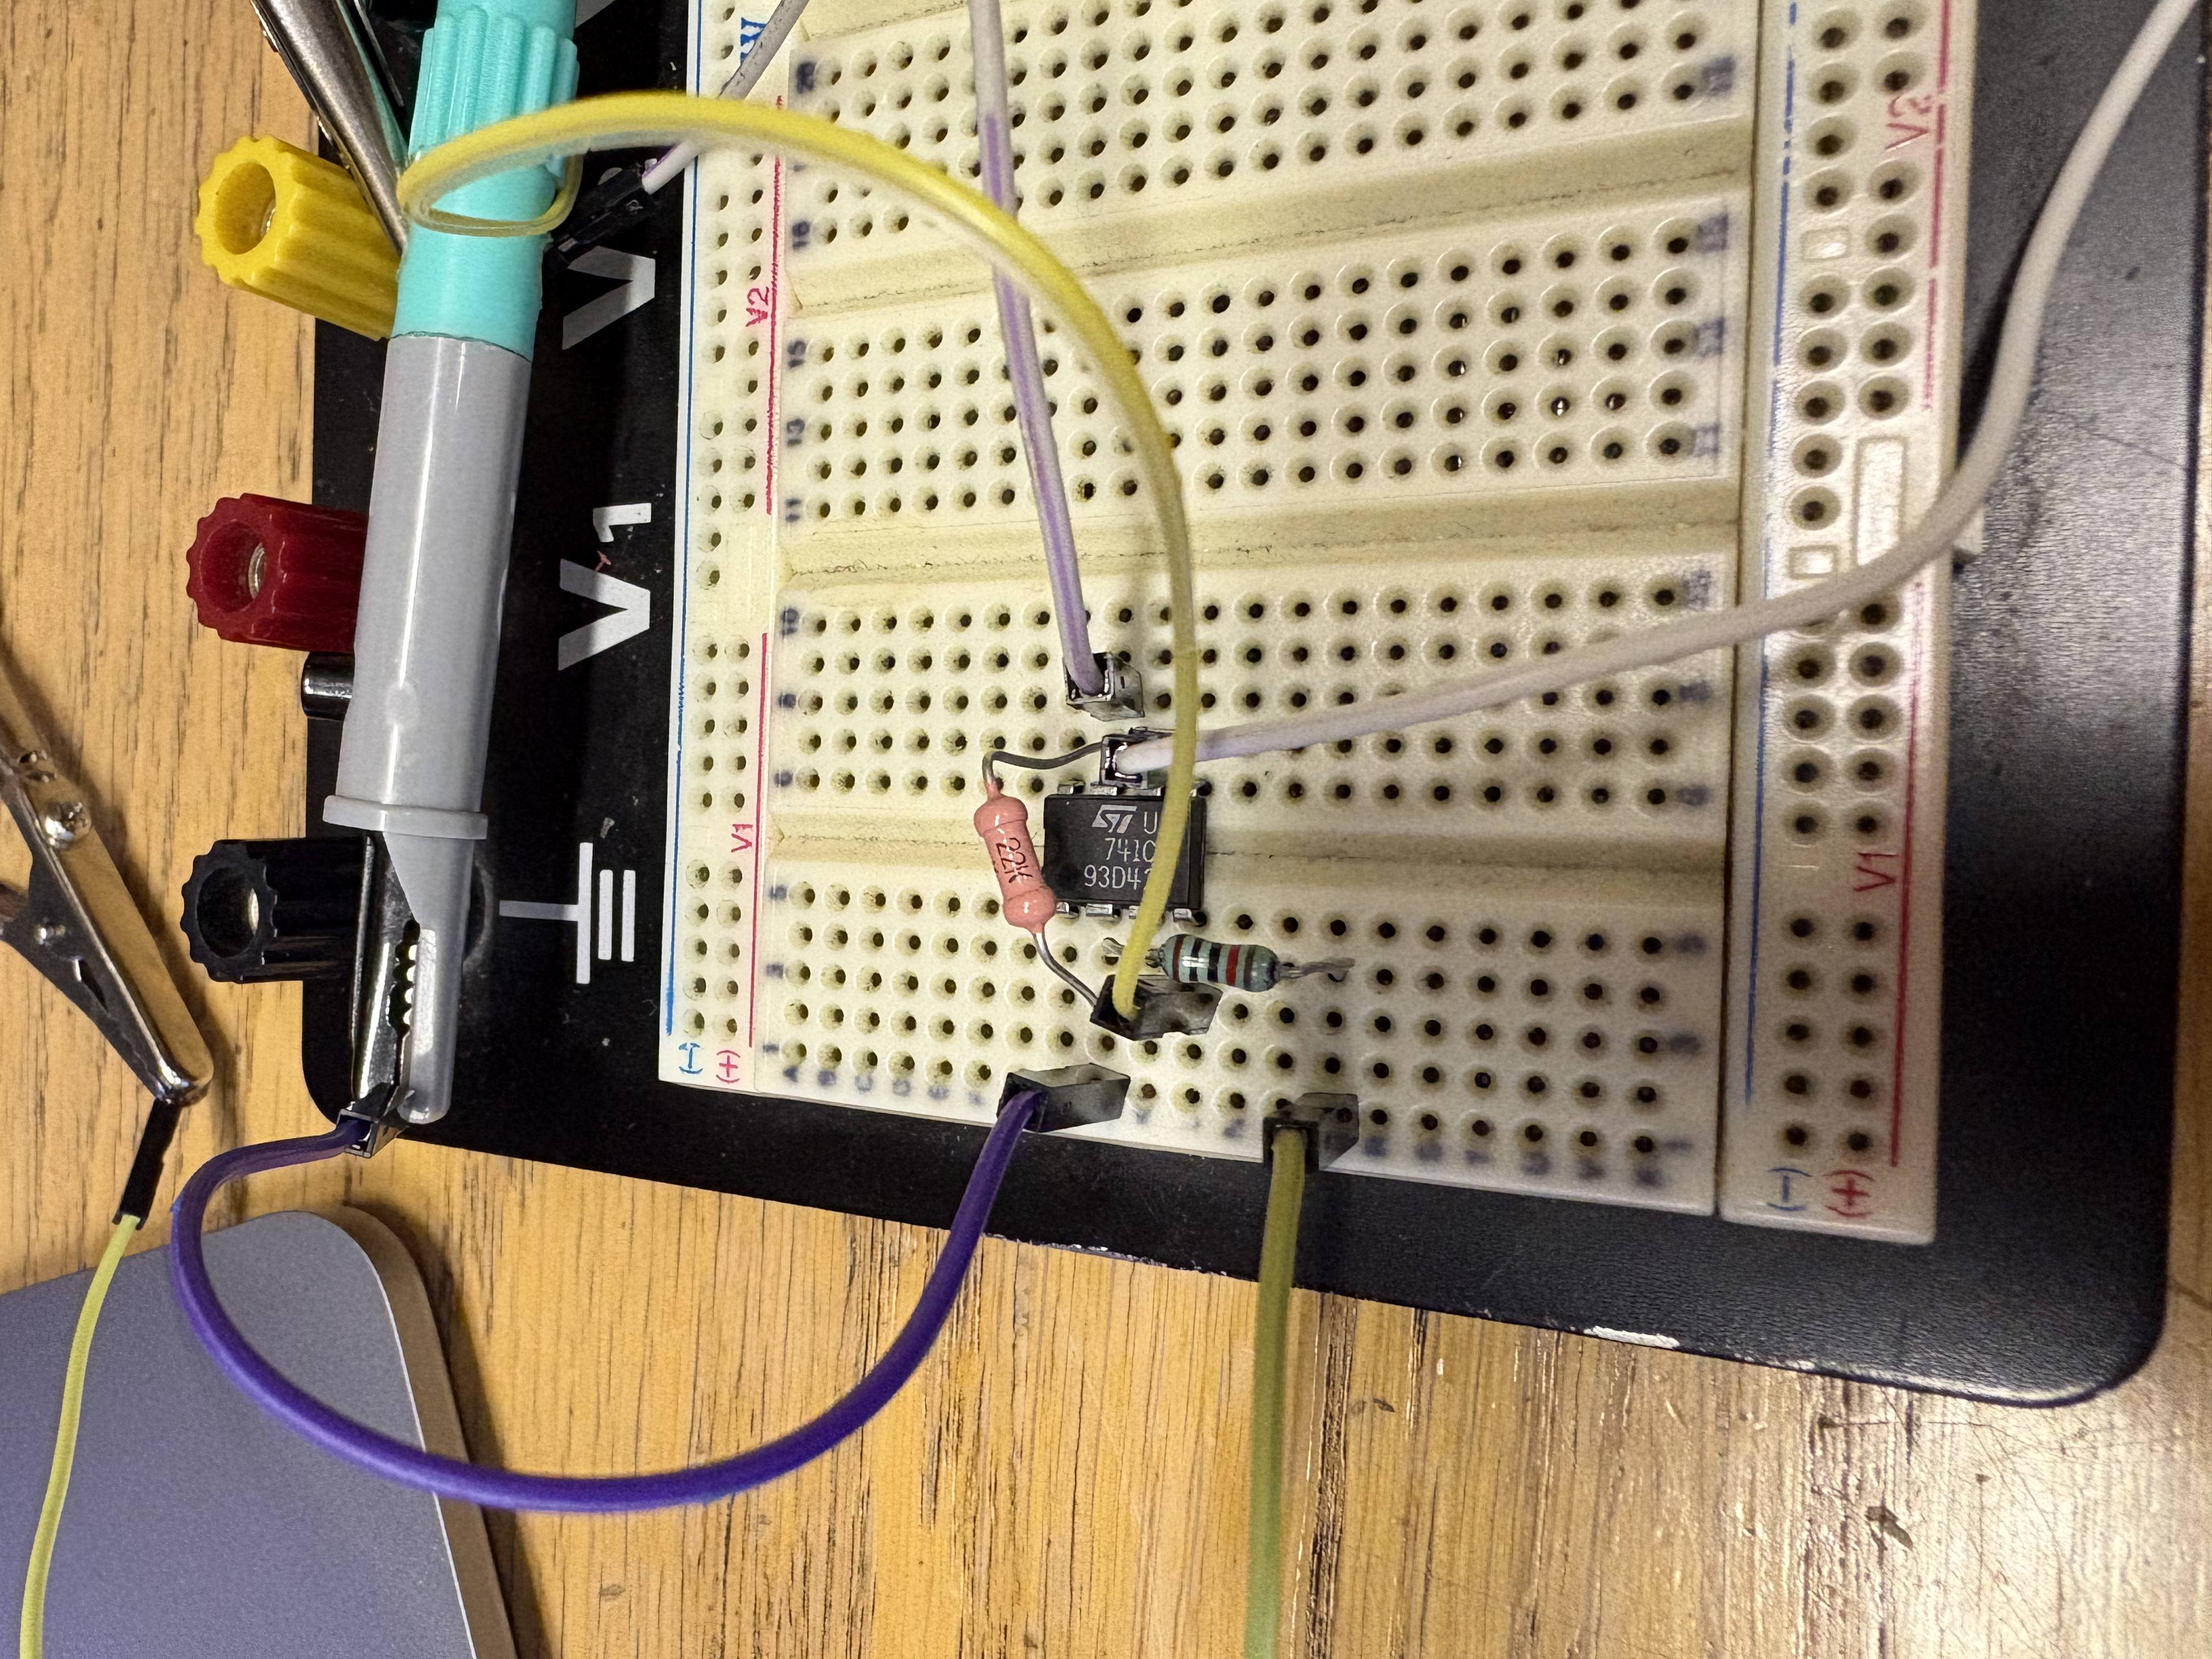
\includegraphics[width=0.5\linewidth]{task1.jpg}
    \caption{Simple comparator setup with two resistors}
    \label{fig:task1}
\end{figure}
We wanted to determine 
the switching threshold of the configuration. We began varying the the voltage, 
satrting from 5V on the input, we found the output to be 4.468V. At this voltage we expected 
the output to be saturated to the positive supply value, which is mostly what we found, 
with a deviation of value:
\newline \begin{center} $ Deviation =\frac{U_{+supp} - U_{out}}{U_{+supp}}=\frac{5 - 4.468}{5}=0.106$ \end{center}
As the configuration acts as a voltage divider on the non-inverting input of 
the operational amplifier, from this we could calculate that we suspect the 
switching threshold to be around:
\newline \begin{center} $ U_{+} =\frac{R_2}{R_1 + R_2}\cdot U_{+supp}=\frac{10}{32}\cdot5=1.5625 V$ \end{center}
Varying the voltage, experimentally we found the switching threshold to be at 
1.6 V, where the output showed -3.058 V on the multimeter. \\
While the measured switching voltage is close to the theoretical value we expected 
at only 2.4\% deviation, we expected the output to saturate to the negative 
supply at -5 V. However, we found that the output went no lower than -3.058 V.\\
We believe this could be because the operational amplifiers we used were not 
rail-to-rail devies. In this case the internal structure of the amplifier is such 
that voltage drops occur on the internal output stage transistors. The asymmetry 
of the voltage drops in the positive and negative saturation regimes can be due 
to the asymmetric output stage on which this voltage drop occurs. \\
The difference we found between the magnitude of the output voltages on the two regimes 
was close to 4.468 - 3.058 = 1.41 V.


\subsection{New switching voltage in Schmitt-trigger with operational amplifier}
Altering the setup of the previous task by adding a resistor of 100 k$\Omega$, 
we created the Schmitt-trigger setup. We expected the switching threshold to extend 
to an interval, as the purpose of the Schmitt-trigger setup was to reduce the sensitivity 
to input noise. We calculated the theoretical switching thresholds to be at:
\begin{gather*}
    U_1 = \frac{5}{1 + \frac{R_1}{R_2} + \frac{R_1}{R_3}} + \frac{U_{\text{out}}}{1 + \frac{R_3}{R_2} + \frac{R_3}{R_1}} = \frac{5\text{ V}}{1 + 2.2 + 0.22} + \frac{U_{\text{out}}}{1 + 10 + 4.545} = 1.462\text{ V} + \frac{U_{\text{out}}}{15.545}\\[1.2em]
    U_{1+} = 1.462\text{ V} + \frac{5\text{ V}}{15.545} = 1.462\text{ V} + 0.322\text{ V} = 1.78\text{ V}\\[1.2em]
    U_{1-} = 1.462\text{ V} + \frac{-5\text{ V}}{15.545} = 1.462\text{ V} - 0.322\text{ V} = 1.14\text{ V}
\end{gather*}
The measured switching thresholds were at 1.8 V and 1.3 V, 
at these thresholds the output switched to -3.086 V and 4.36 V respectively. 
The higher threshold - below which the output voltage saturates to the negative supply 
voltage - is very close to the theoretical value, with only 1\% deviation. The lower 
threshold - where the output saturated to the positive supply voltage - deviated by 14\%. 
We believe this signification deviation could also be a result of the resolution of 
the measurement device used. We could only be precise to 1 decimal point, at which point 
the deviation could have also been 9\% at 1.25 V on the input, rounded up to 1.3 V.\\
The difference between the output voltage magnitudes stayed relatively unchanged, compared 
to the previous task.

\subsection{Waveforms of the relaxation oscillator with operational amplifier}

\begin{figure}[H]
    \centering
    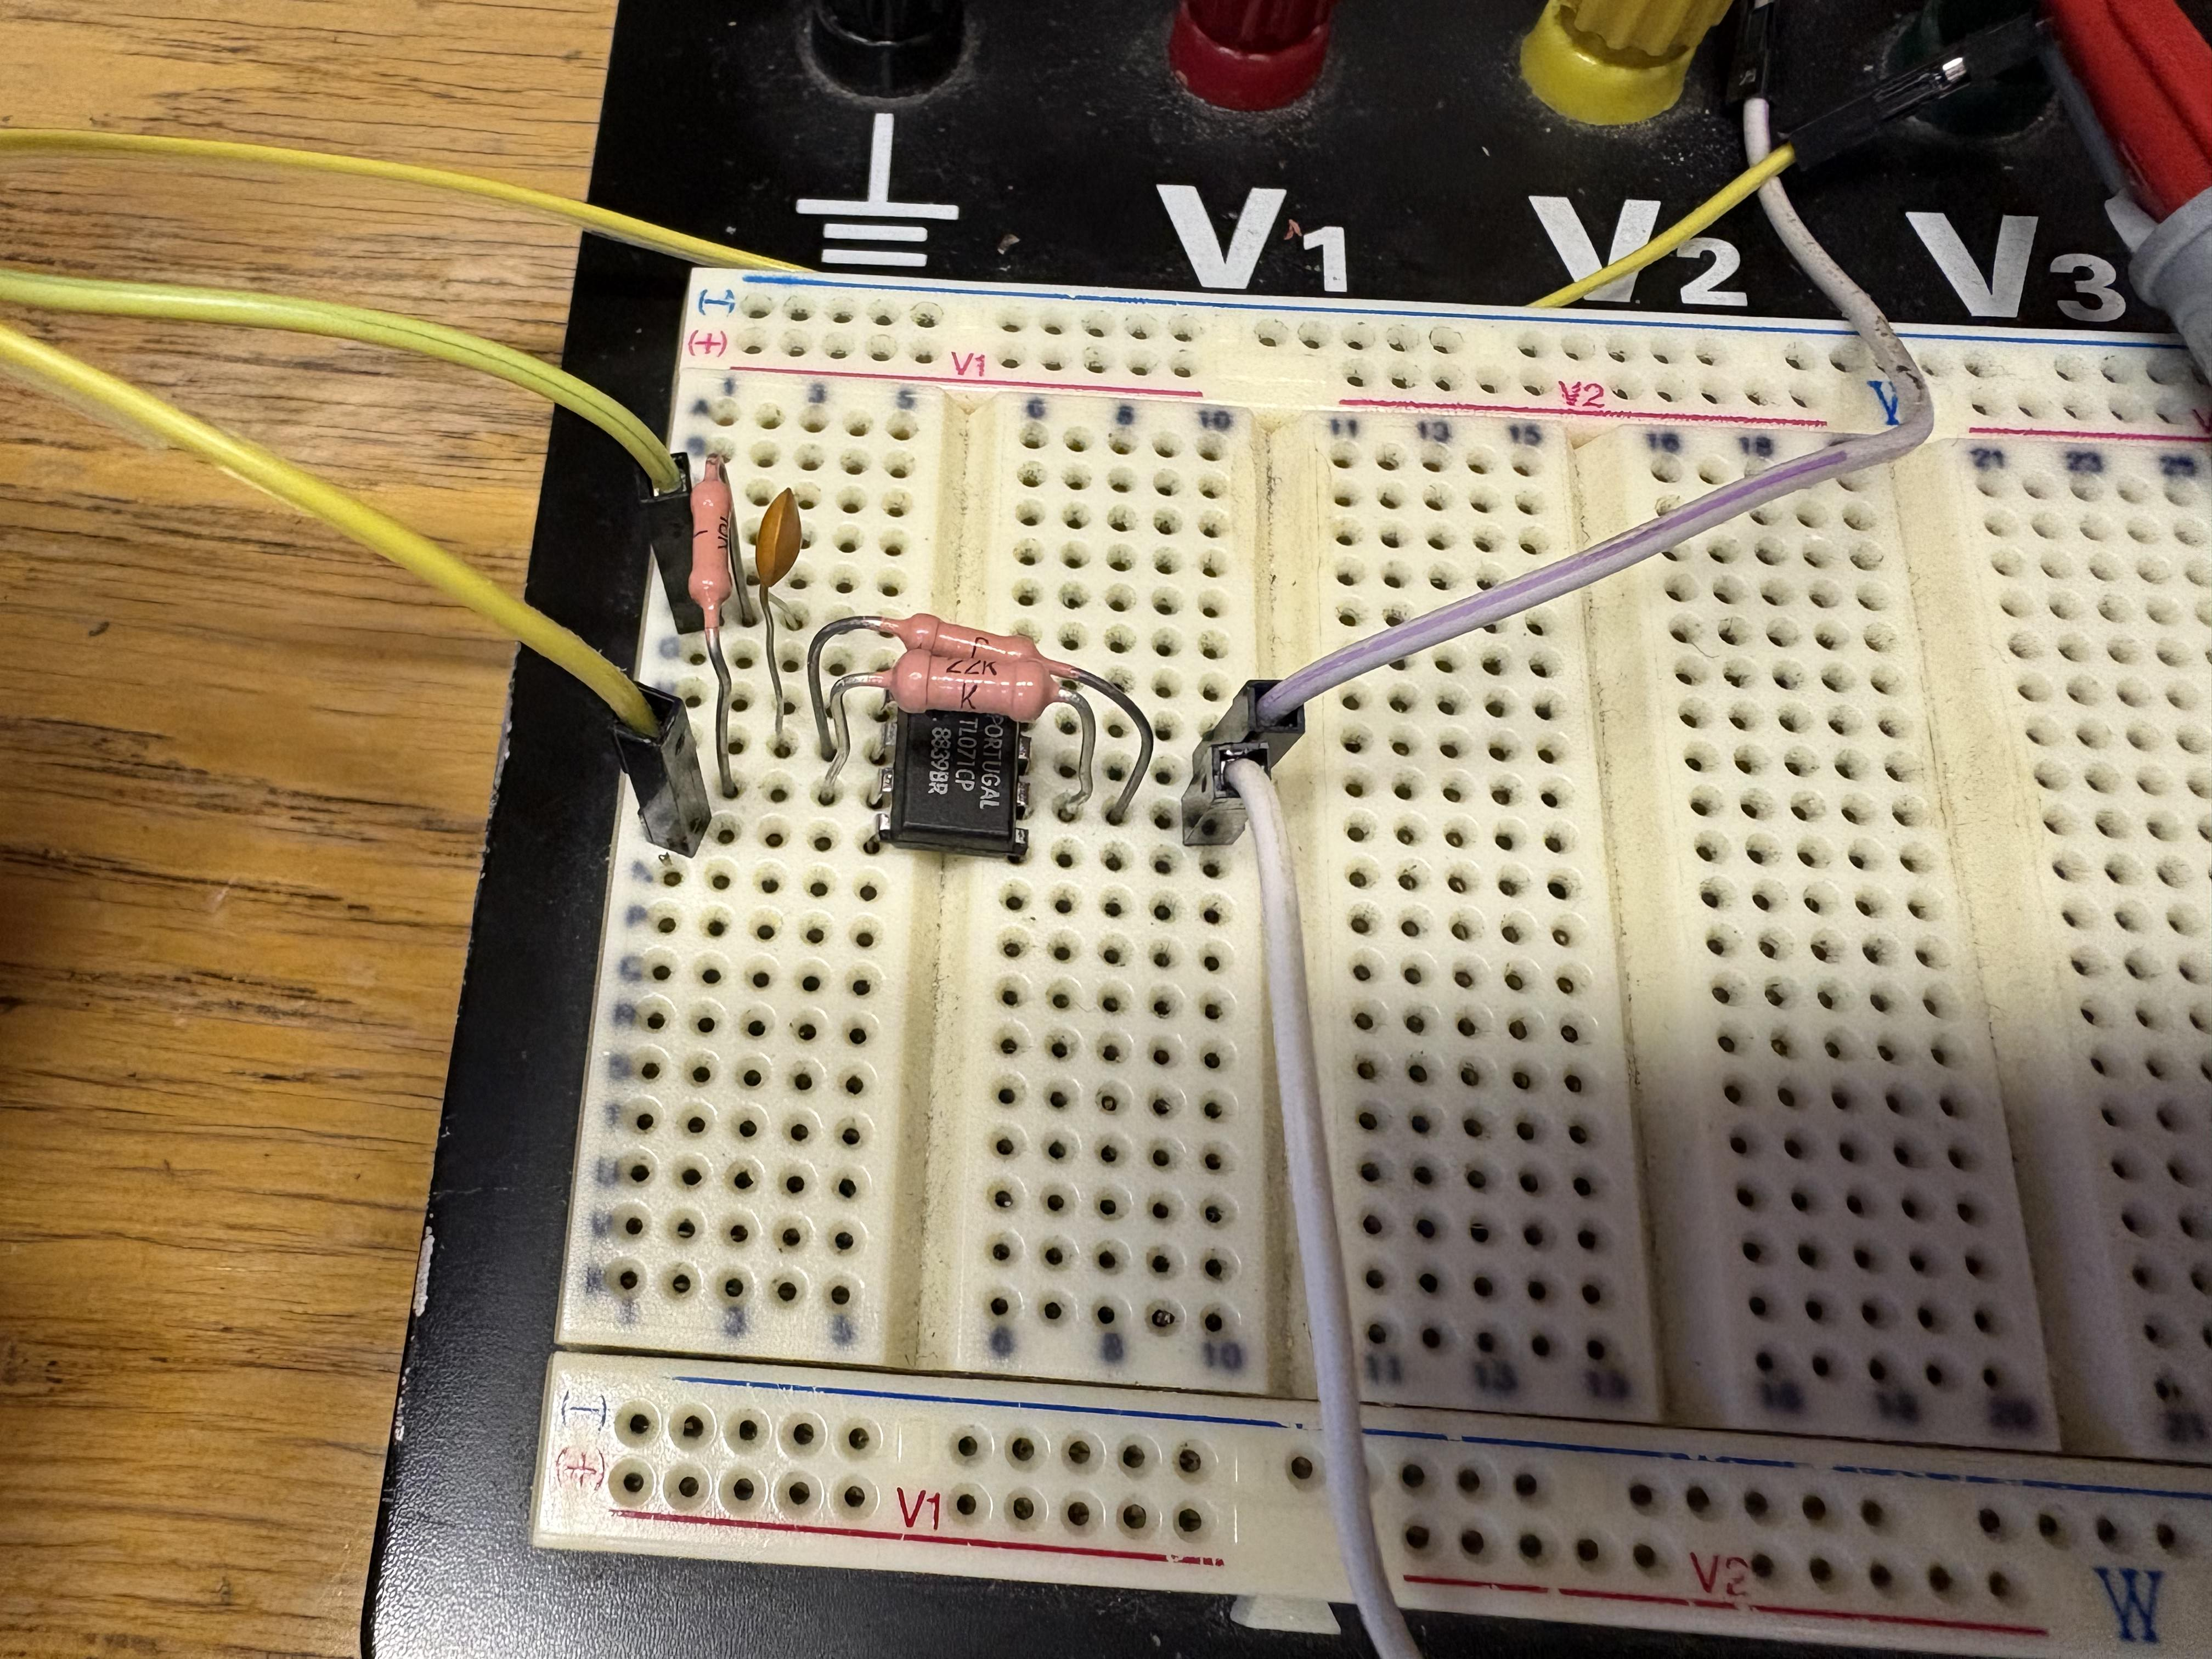
\includegraphics[width=0.5\linewidth]{task3.jpg}
    \caption{Relaxation oscillator setup with three resistors and one capacitor}
    \label{fig:task3}
\end{figure}
To determine the value of the capacitance we needed to use in the relaxed oscillator setup, 
we used the following equations first to find the switching voltages, and then to determine 
the capacitance through the period equation knowing that the period is the inverse of the 
frequency:
\begin{gather*}
    U_{1s1} = U_+ \cdot \frac{R_2}{R_2 + R_3} \quad \text{and} \quad U_{1s2} = U_- \cdot \frac{R_2}{R_2 + R_3}\\[1.2em]
    T = 2 \cdot R_1 \cdot C \cdot \ln\left( \frac{U_+ + U_{1s1}}{U_+ + U_{1s2}} \right)\\[1.2em]
    C = \frac{1}{2 \cdot f \cdot R_1 \cdot \ln\left( 1 + \frac{2 R_2}{R_3} \right)} = 6.49 \text{ nF}
\end{gather*}

The capacitor with the closes value we found was that of 6.8 nF. Beginning with the 
TL071CP operational amplifier (seen in figure 3a, b, and c) we checked the waveform shapes 
of inputs and outputs, then we repeated this with the $\mu$A741CN operational amplifier 
(figure 3d, e, f). The observed shapes of the waveforms are summarised in the table below:

\begin{table}[H]
    \centering
    \label{tab:relaxed}
    \begin{tabular}{|c|c|c|c|}
        \hline
        Operational Amplifier & U1 & U2 & Uo \\
        \hline
        TL071CP & Square & Triangle & Square  \\
        \hline
        $\mu$A741CN & Trapeze & Soft triangle & Trapeze  \\
        \hline
    \end{tabular}
    \caption{Observed waveforms of the noninverting (U1), inverting (U2), and output (Uo) signals with TL071CP and $\mu$A741CN operational amplifiers.}
\end{table}

\begin{figure}[H]
    \centering
    % Row 1: TL
    \begin{subfigure}{0.48\textwidth}
        \centering
        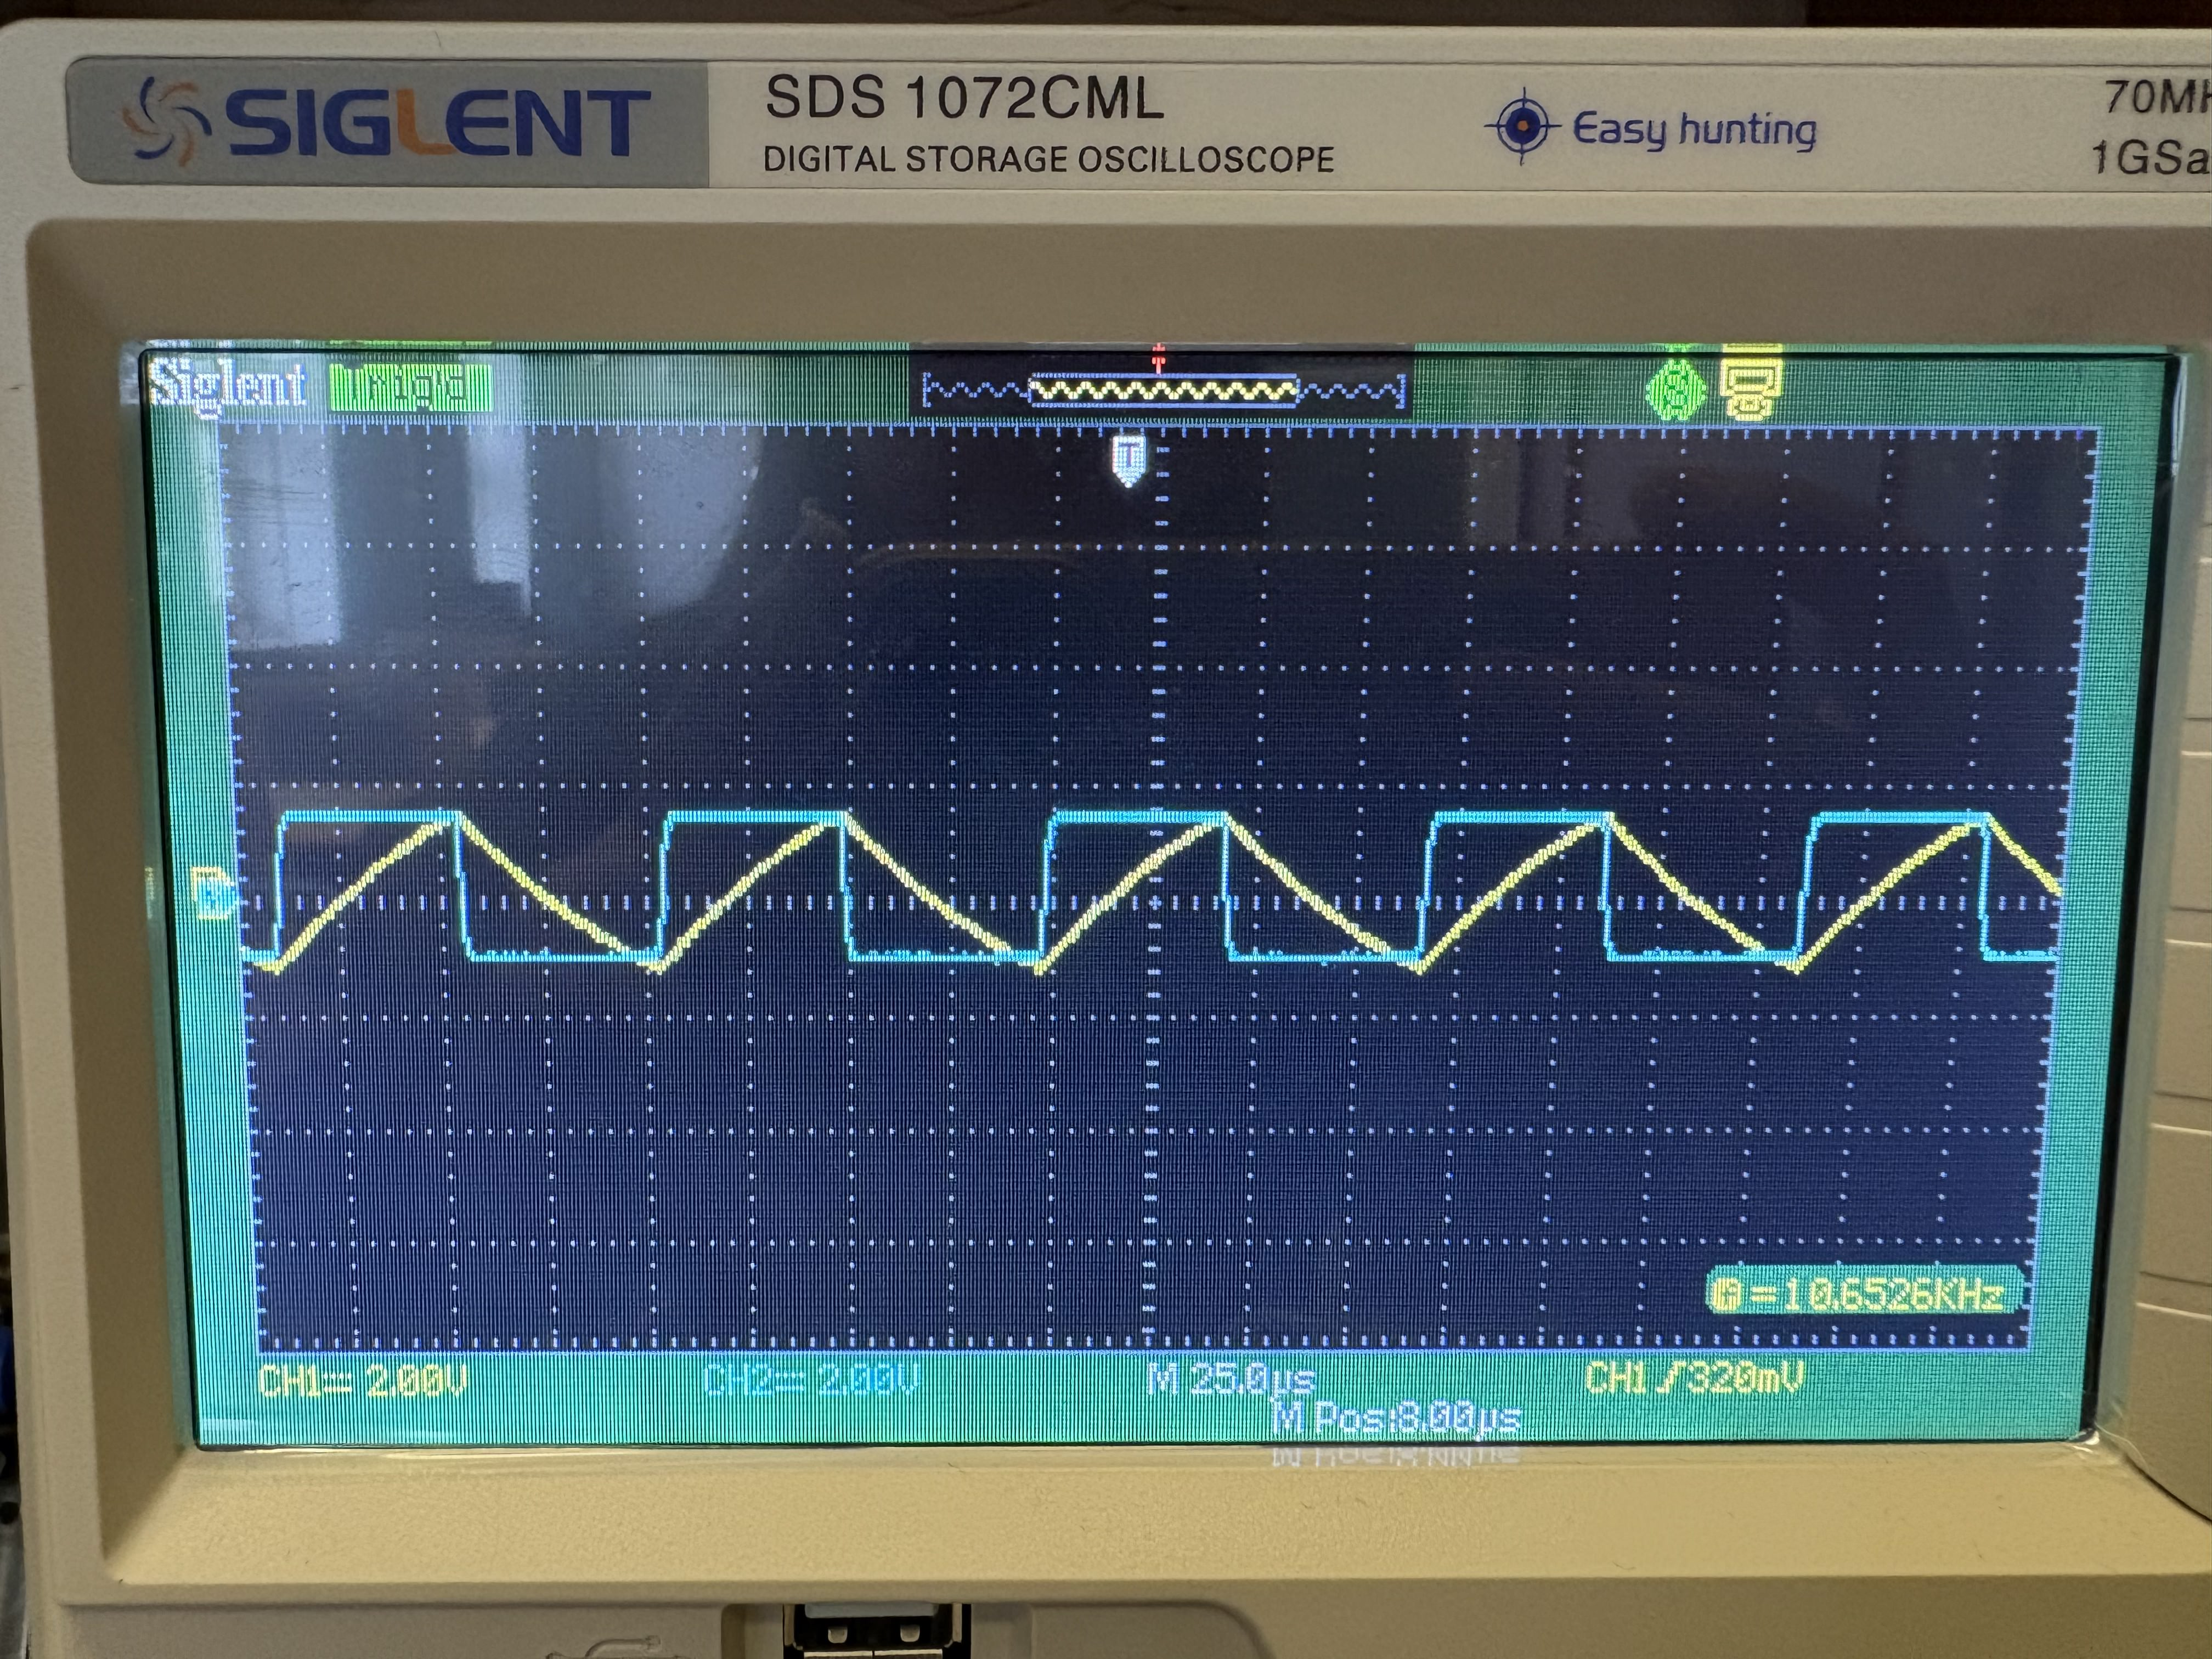
\includegraphics[width=\linewidth]{U1_U2_TL.jpg}
        \caption{TL: Measurement of U$_{1}$ on channel 2 and U$_{2}$ on channel 1}
    \end{subfigure}
    \hfill
    \begin{subfigure}{0.48\textwidth}
        \centering
        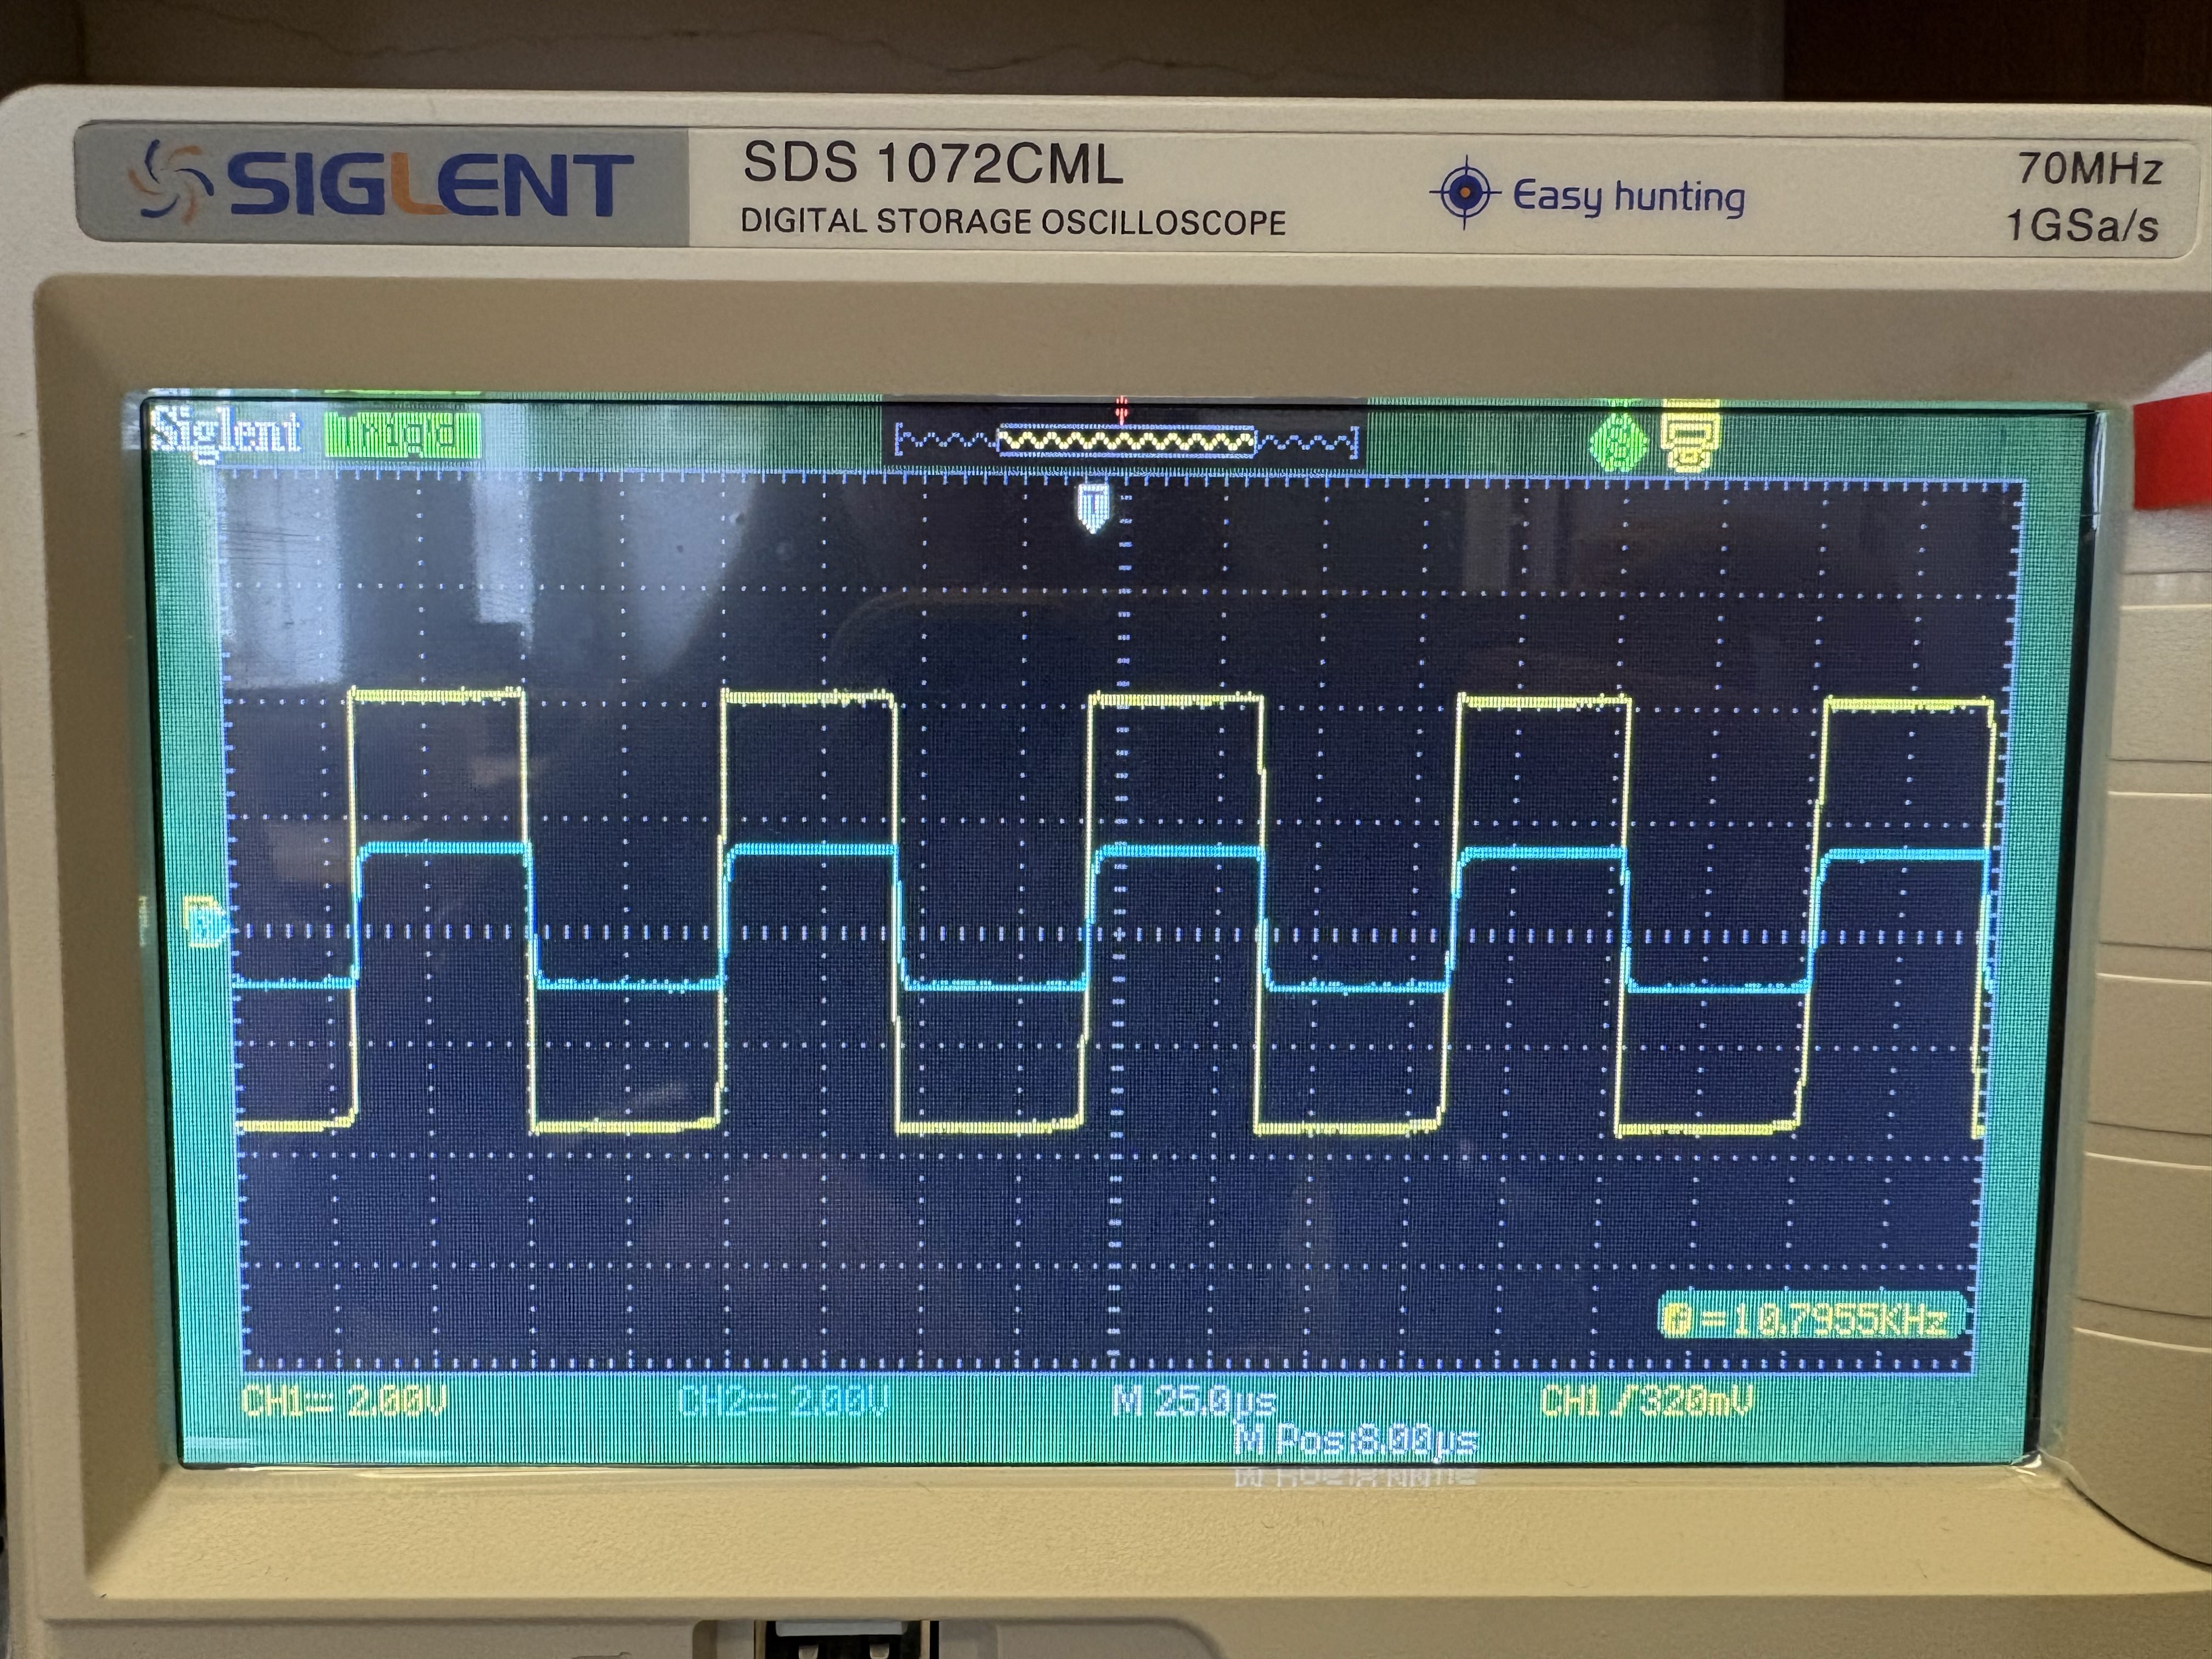
\includegraphics[width=\linewidth]{U1_Uo_TL.jpg}
        \caption{TL: Measurement of U$_{1}$ on channel 2 and U$_{out}$ on channel 1}
    \end{subfigure}

    \vspace{0.3cm}

    % Row 2: TL and AU
    \begin{subfigure}{0.48\textwidth}
        \centering
        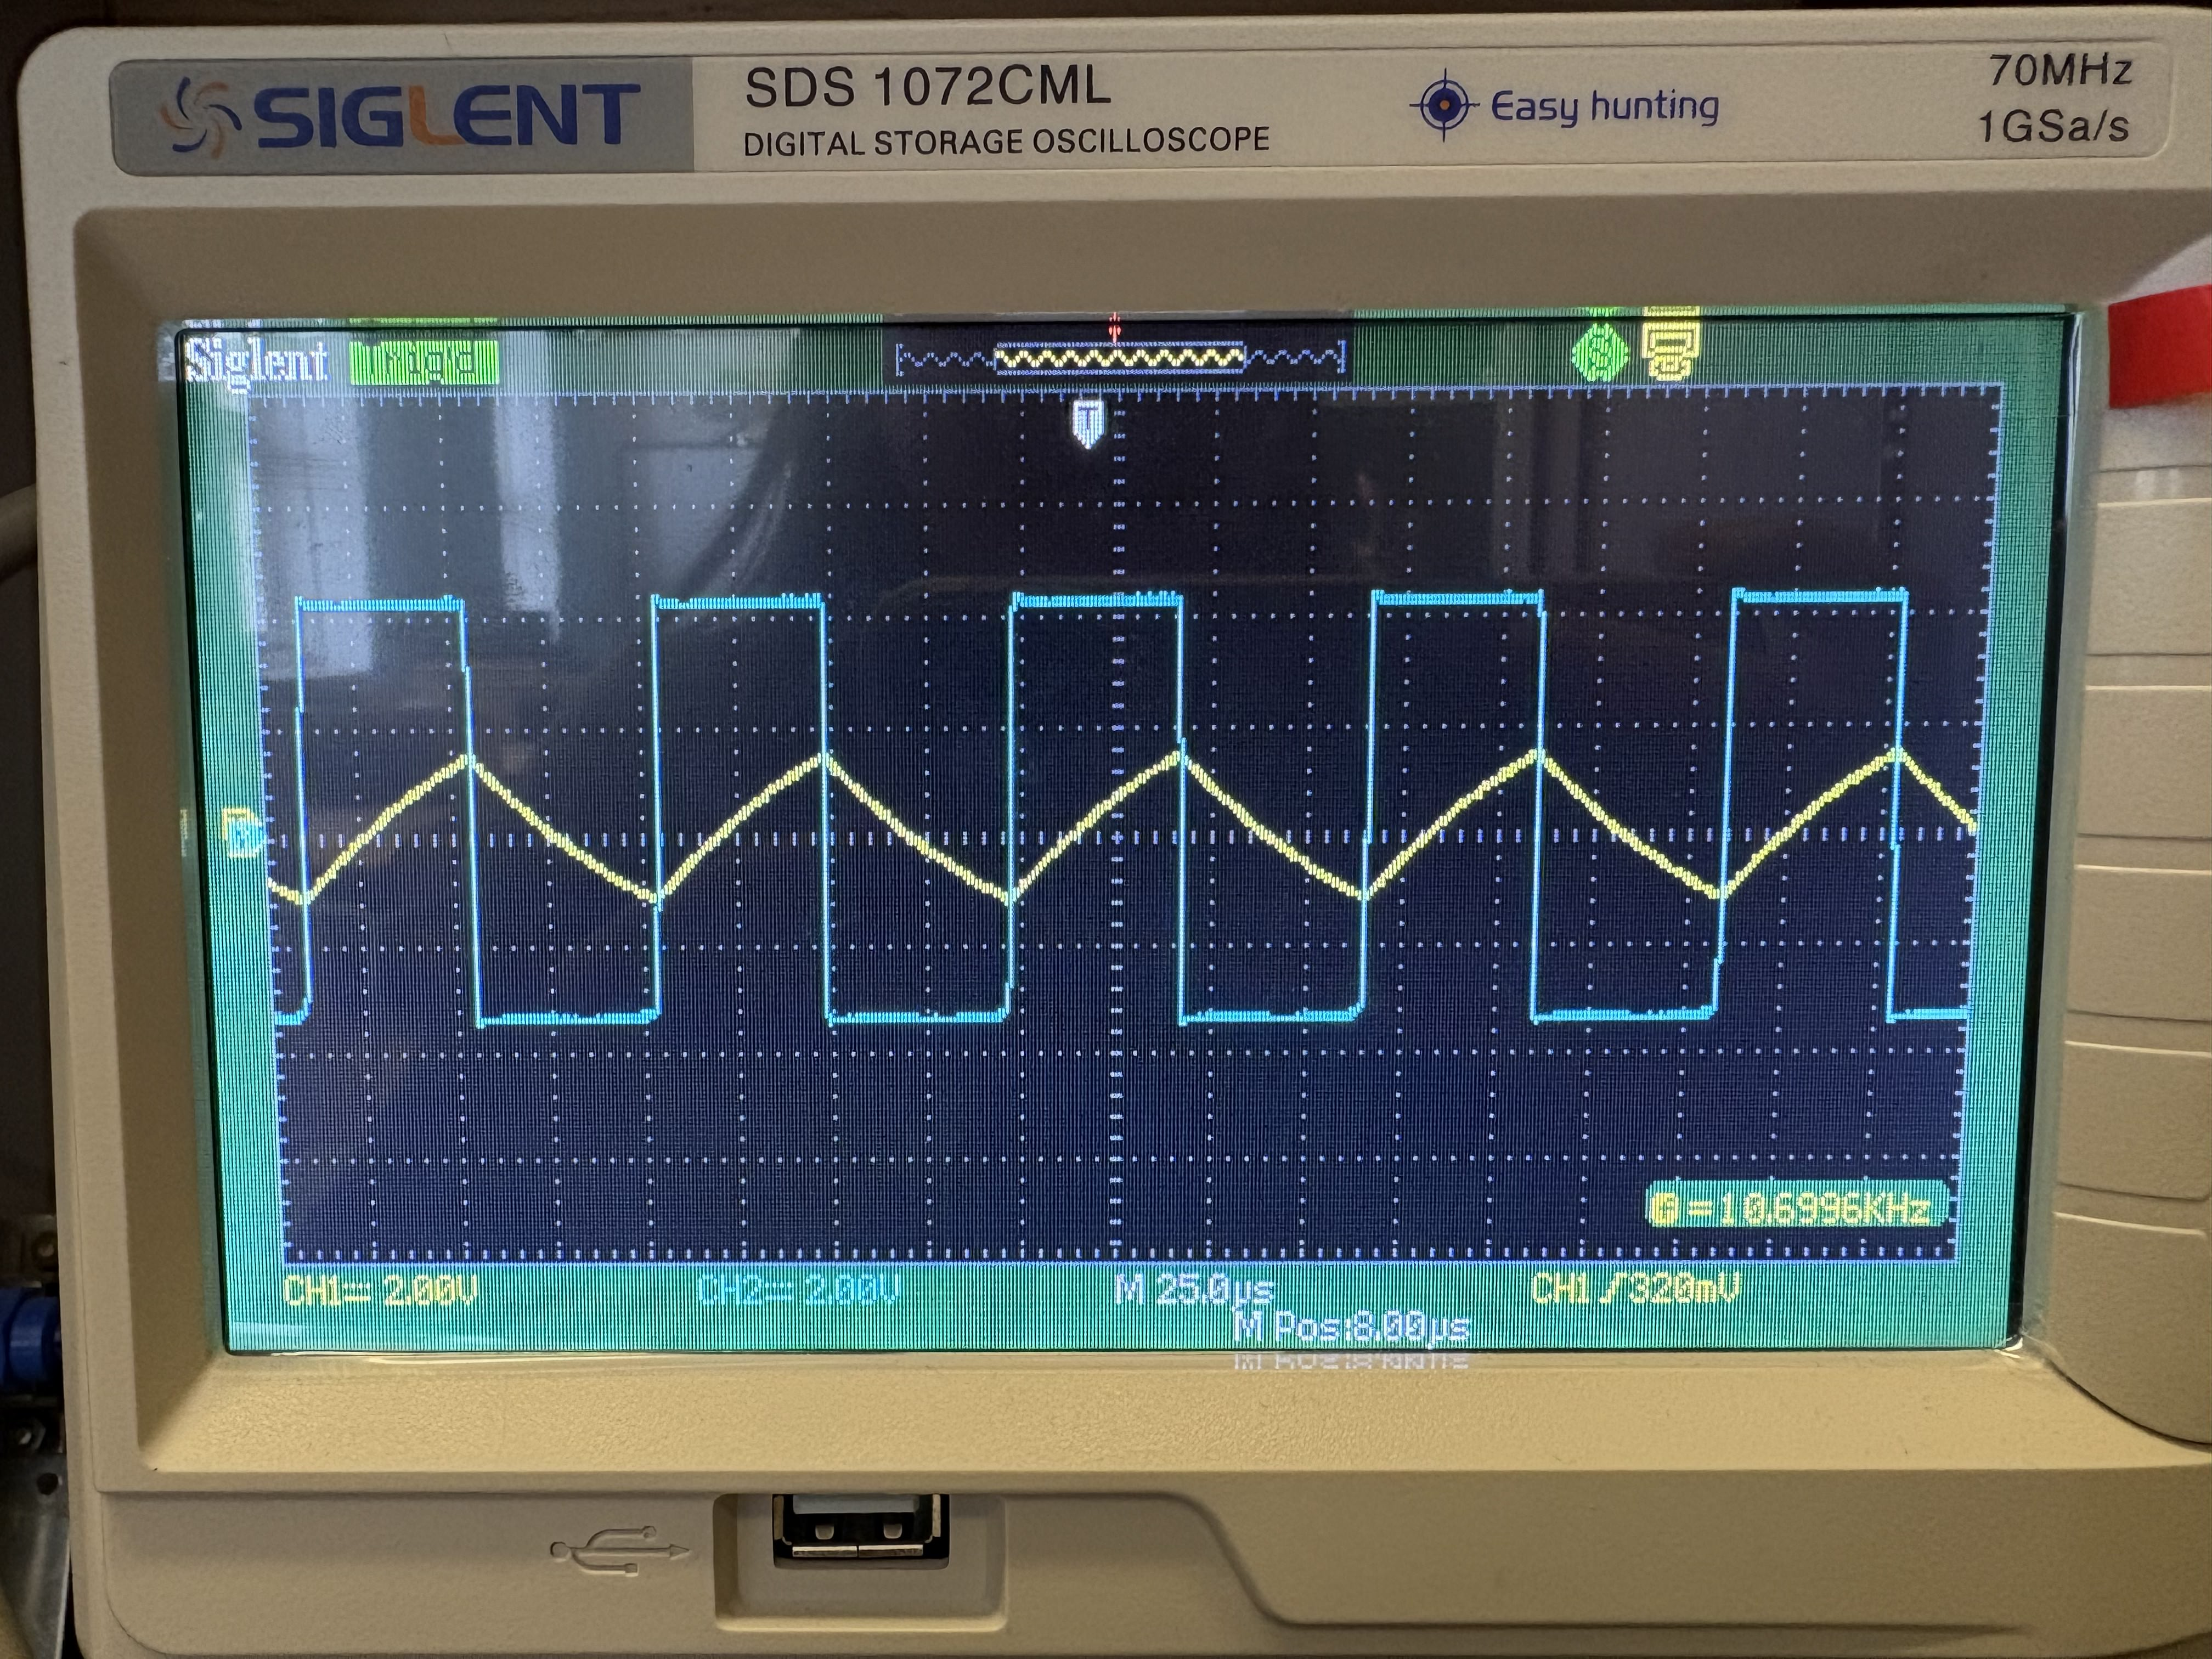
\includegraphics[width=\linewidth]{U2_Uo_TL.jpg}
        \caption{TL: Measurement of U$_{out}$ on channel 2 and U$_{2}$ on channel 1}
    \end{subfigure}
    \hfill
    \begin{subfigure}{0.48\textwidth}
        \centering
        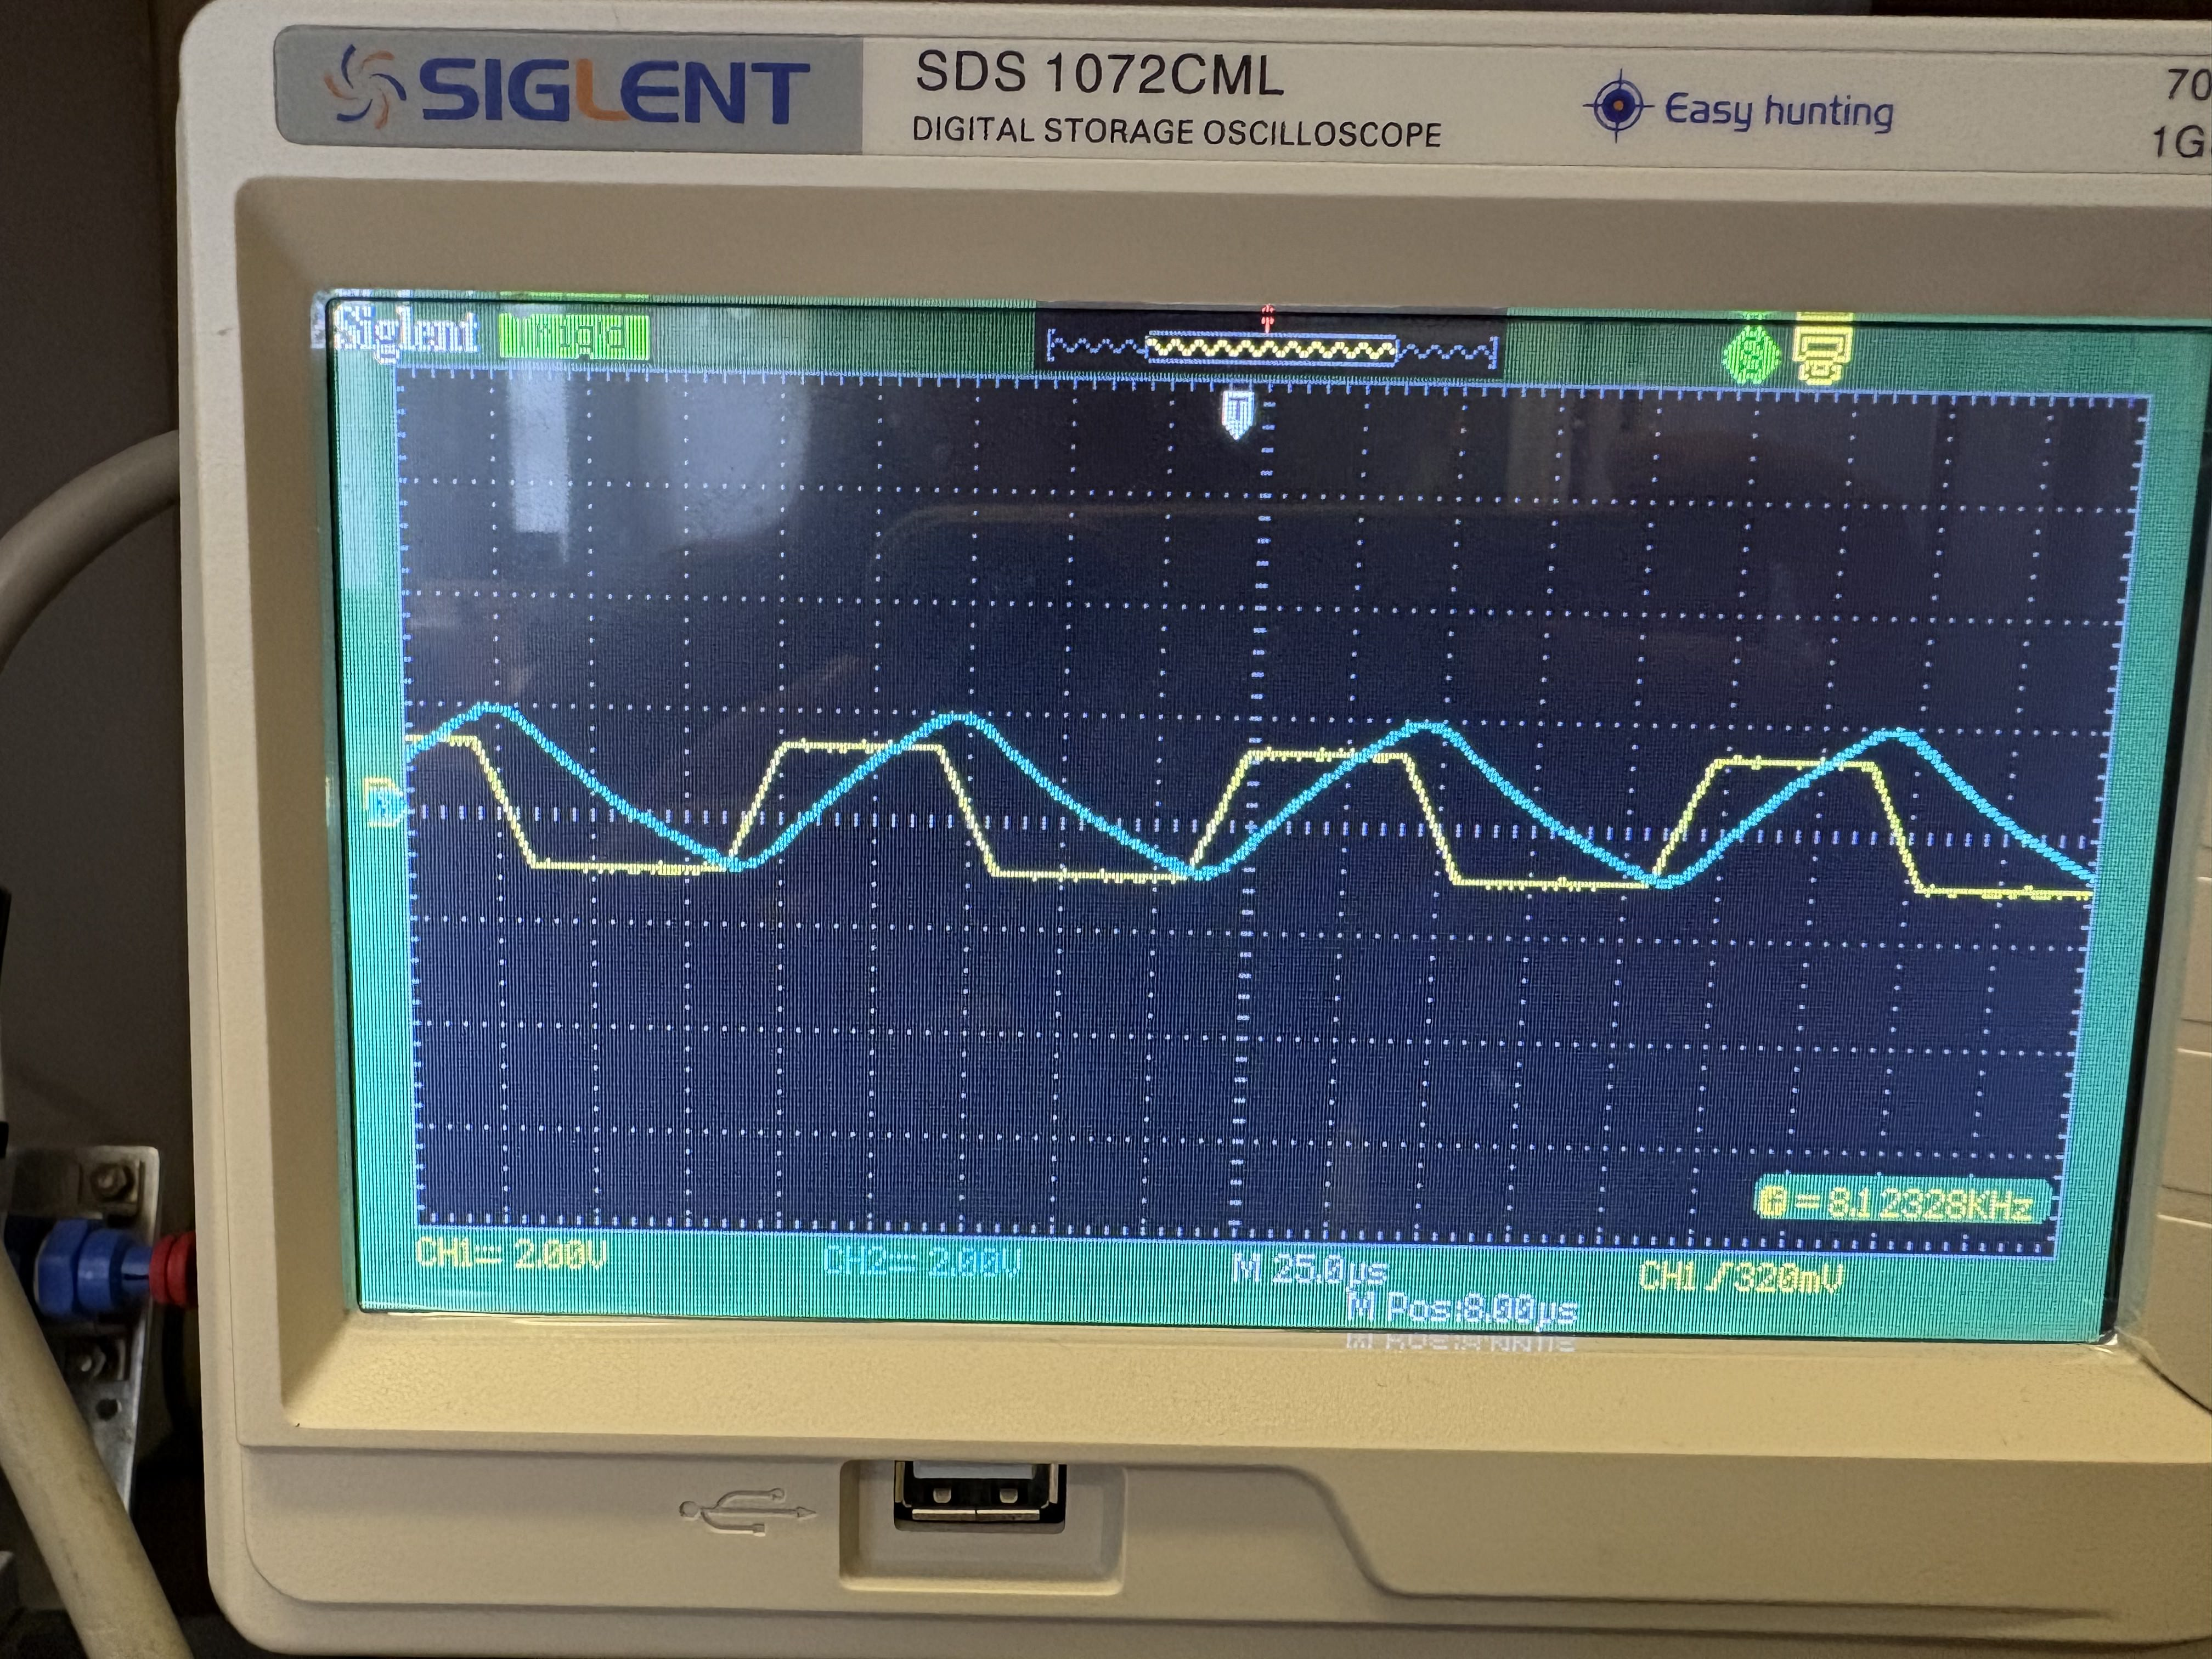
\includegraphics[width=\linewidth]{U1_U2_AU.jpg}
        \caption{AU: Measurement of U$_{2}$ on channel 2 and U$_{1}$ on channel 1}
    \end{subfigure}

    \vspace{0.3cm}

    % Row 3: AU
    \begin{subfigure}{0.48\textwidth}
        \centering
        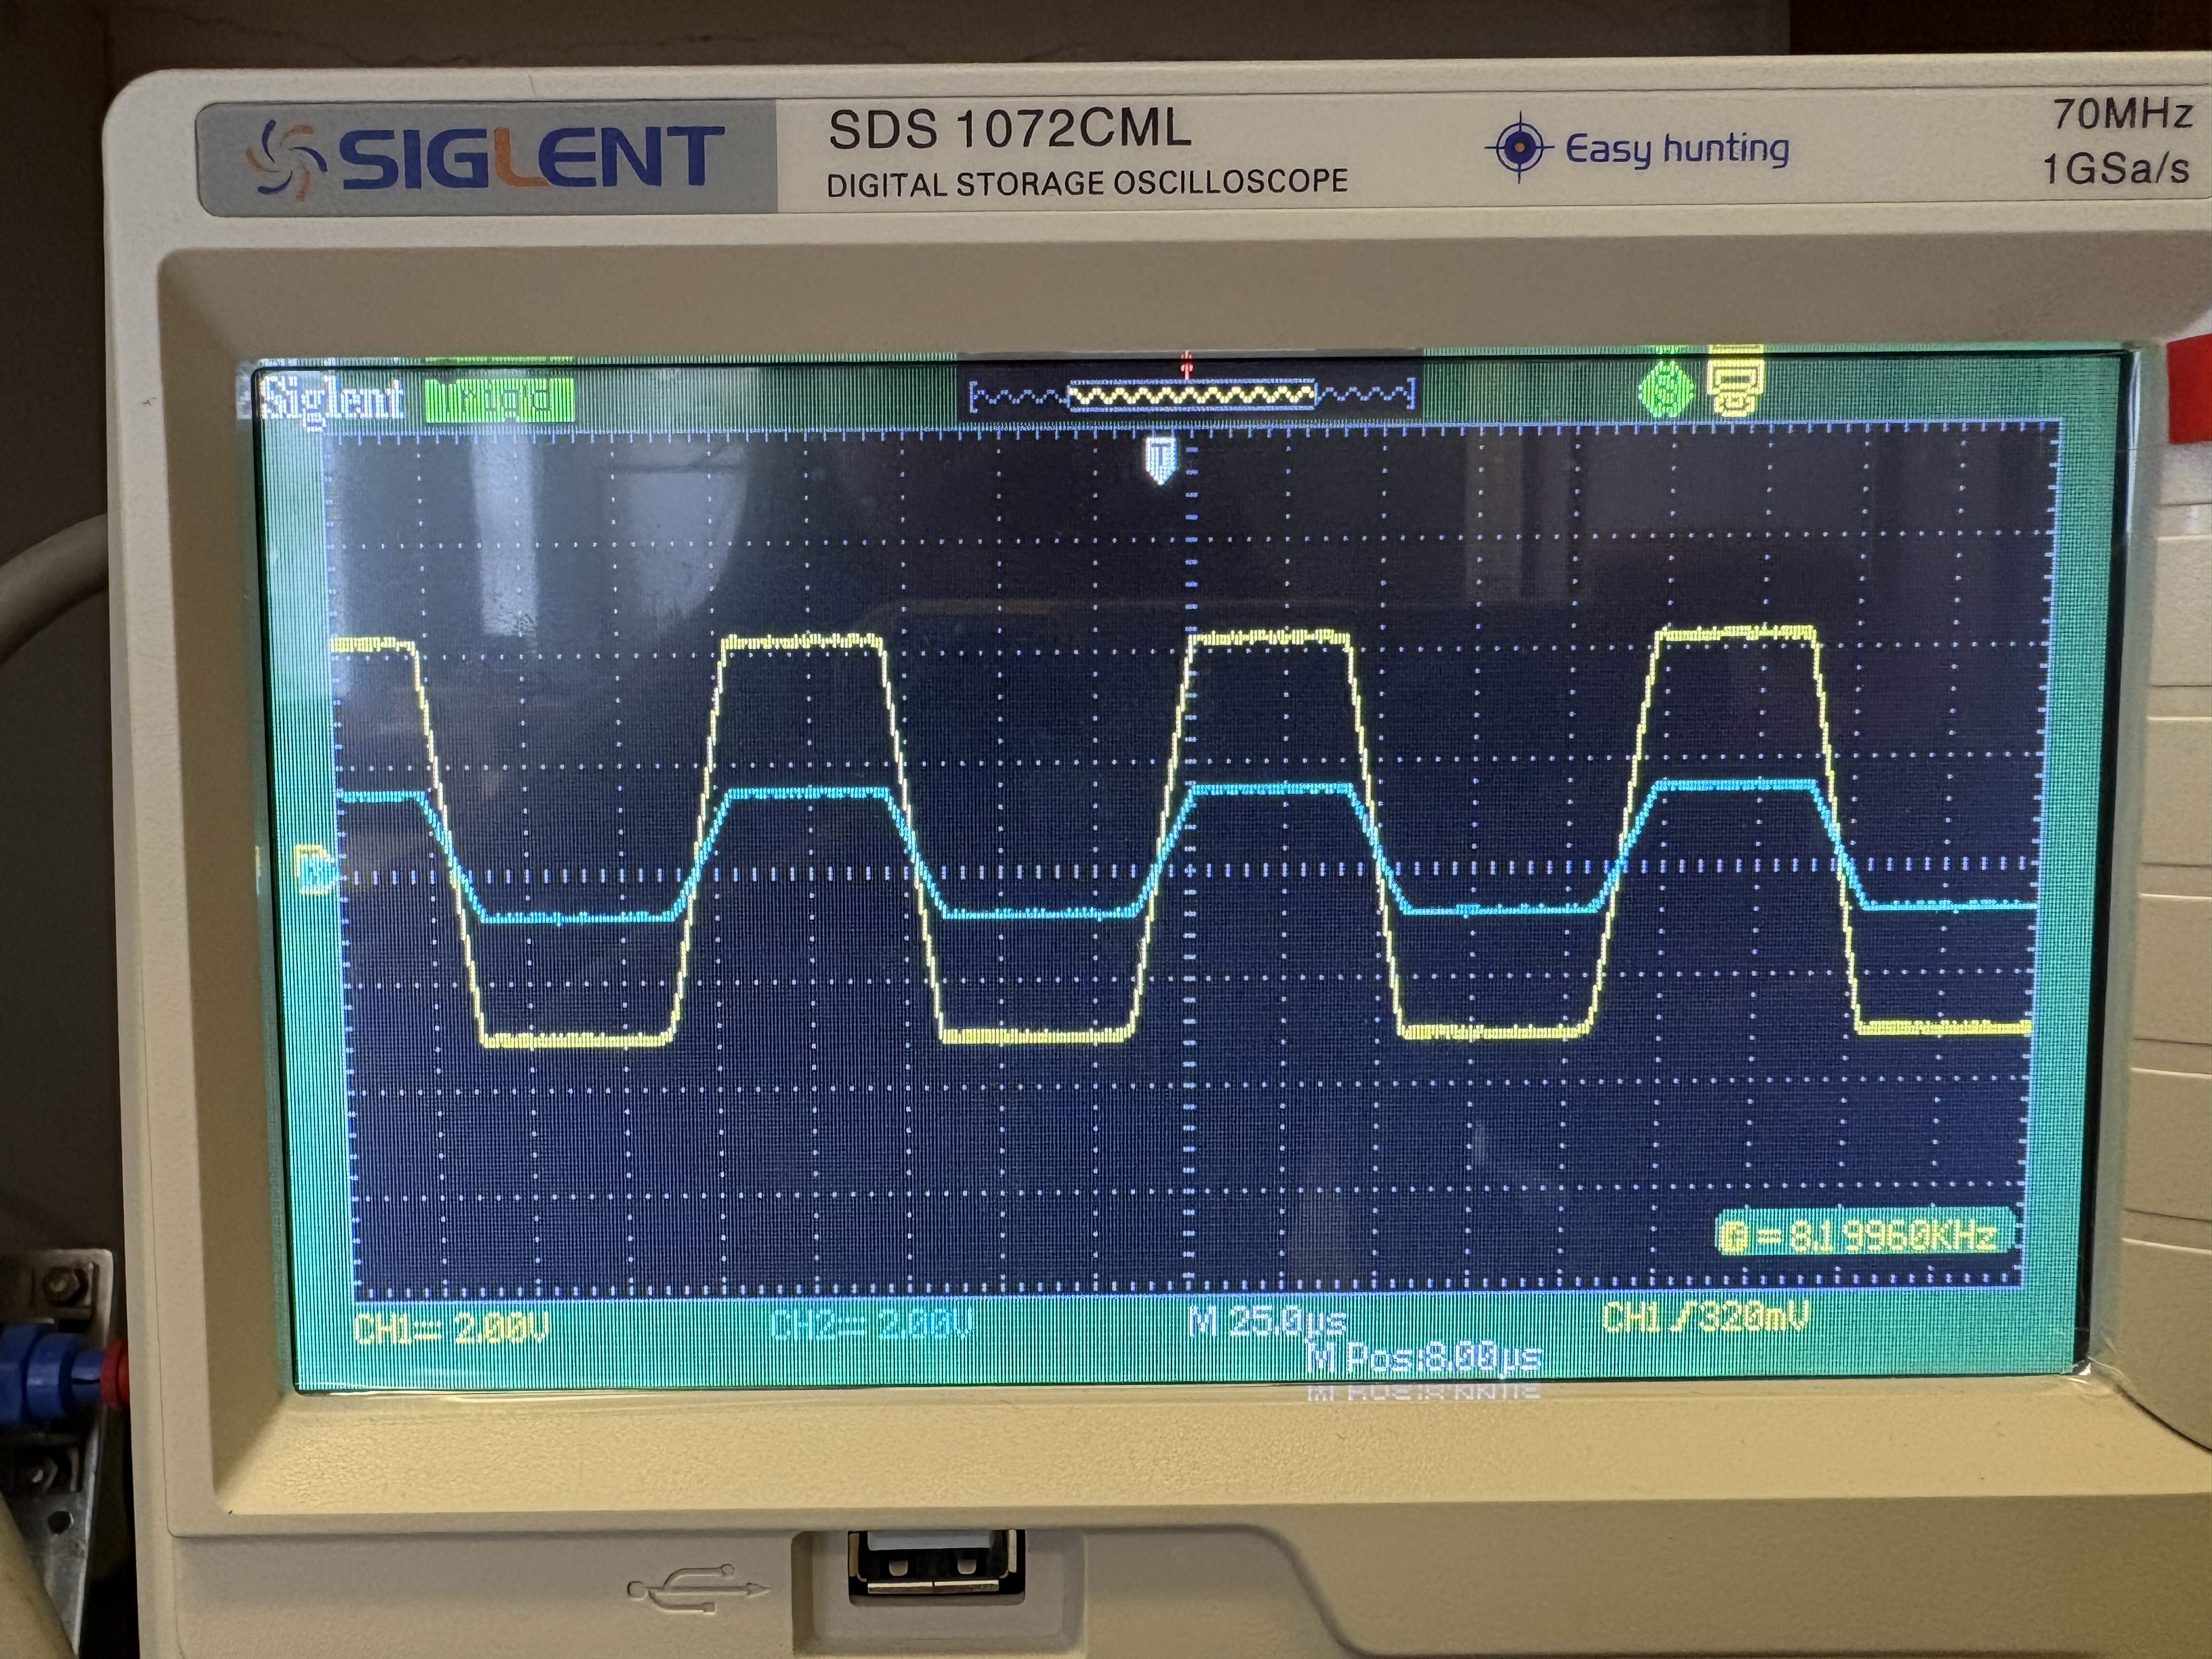
\includegraphics[width=\linewidth]{U1_Uo_AU.jpg}
        \caption{AU: Measurement of U$_{1}$ on channel 2 and U$_{out}$ on channel 1}
    \end{subfigure}
    \hfill
    \begin{subfigure}{0.48\textwidth}
        \centering
        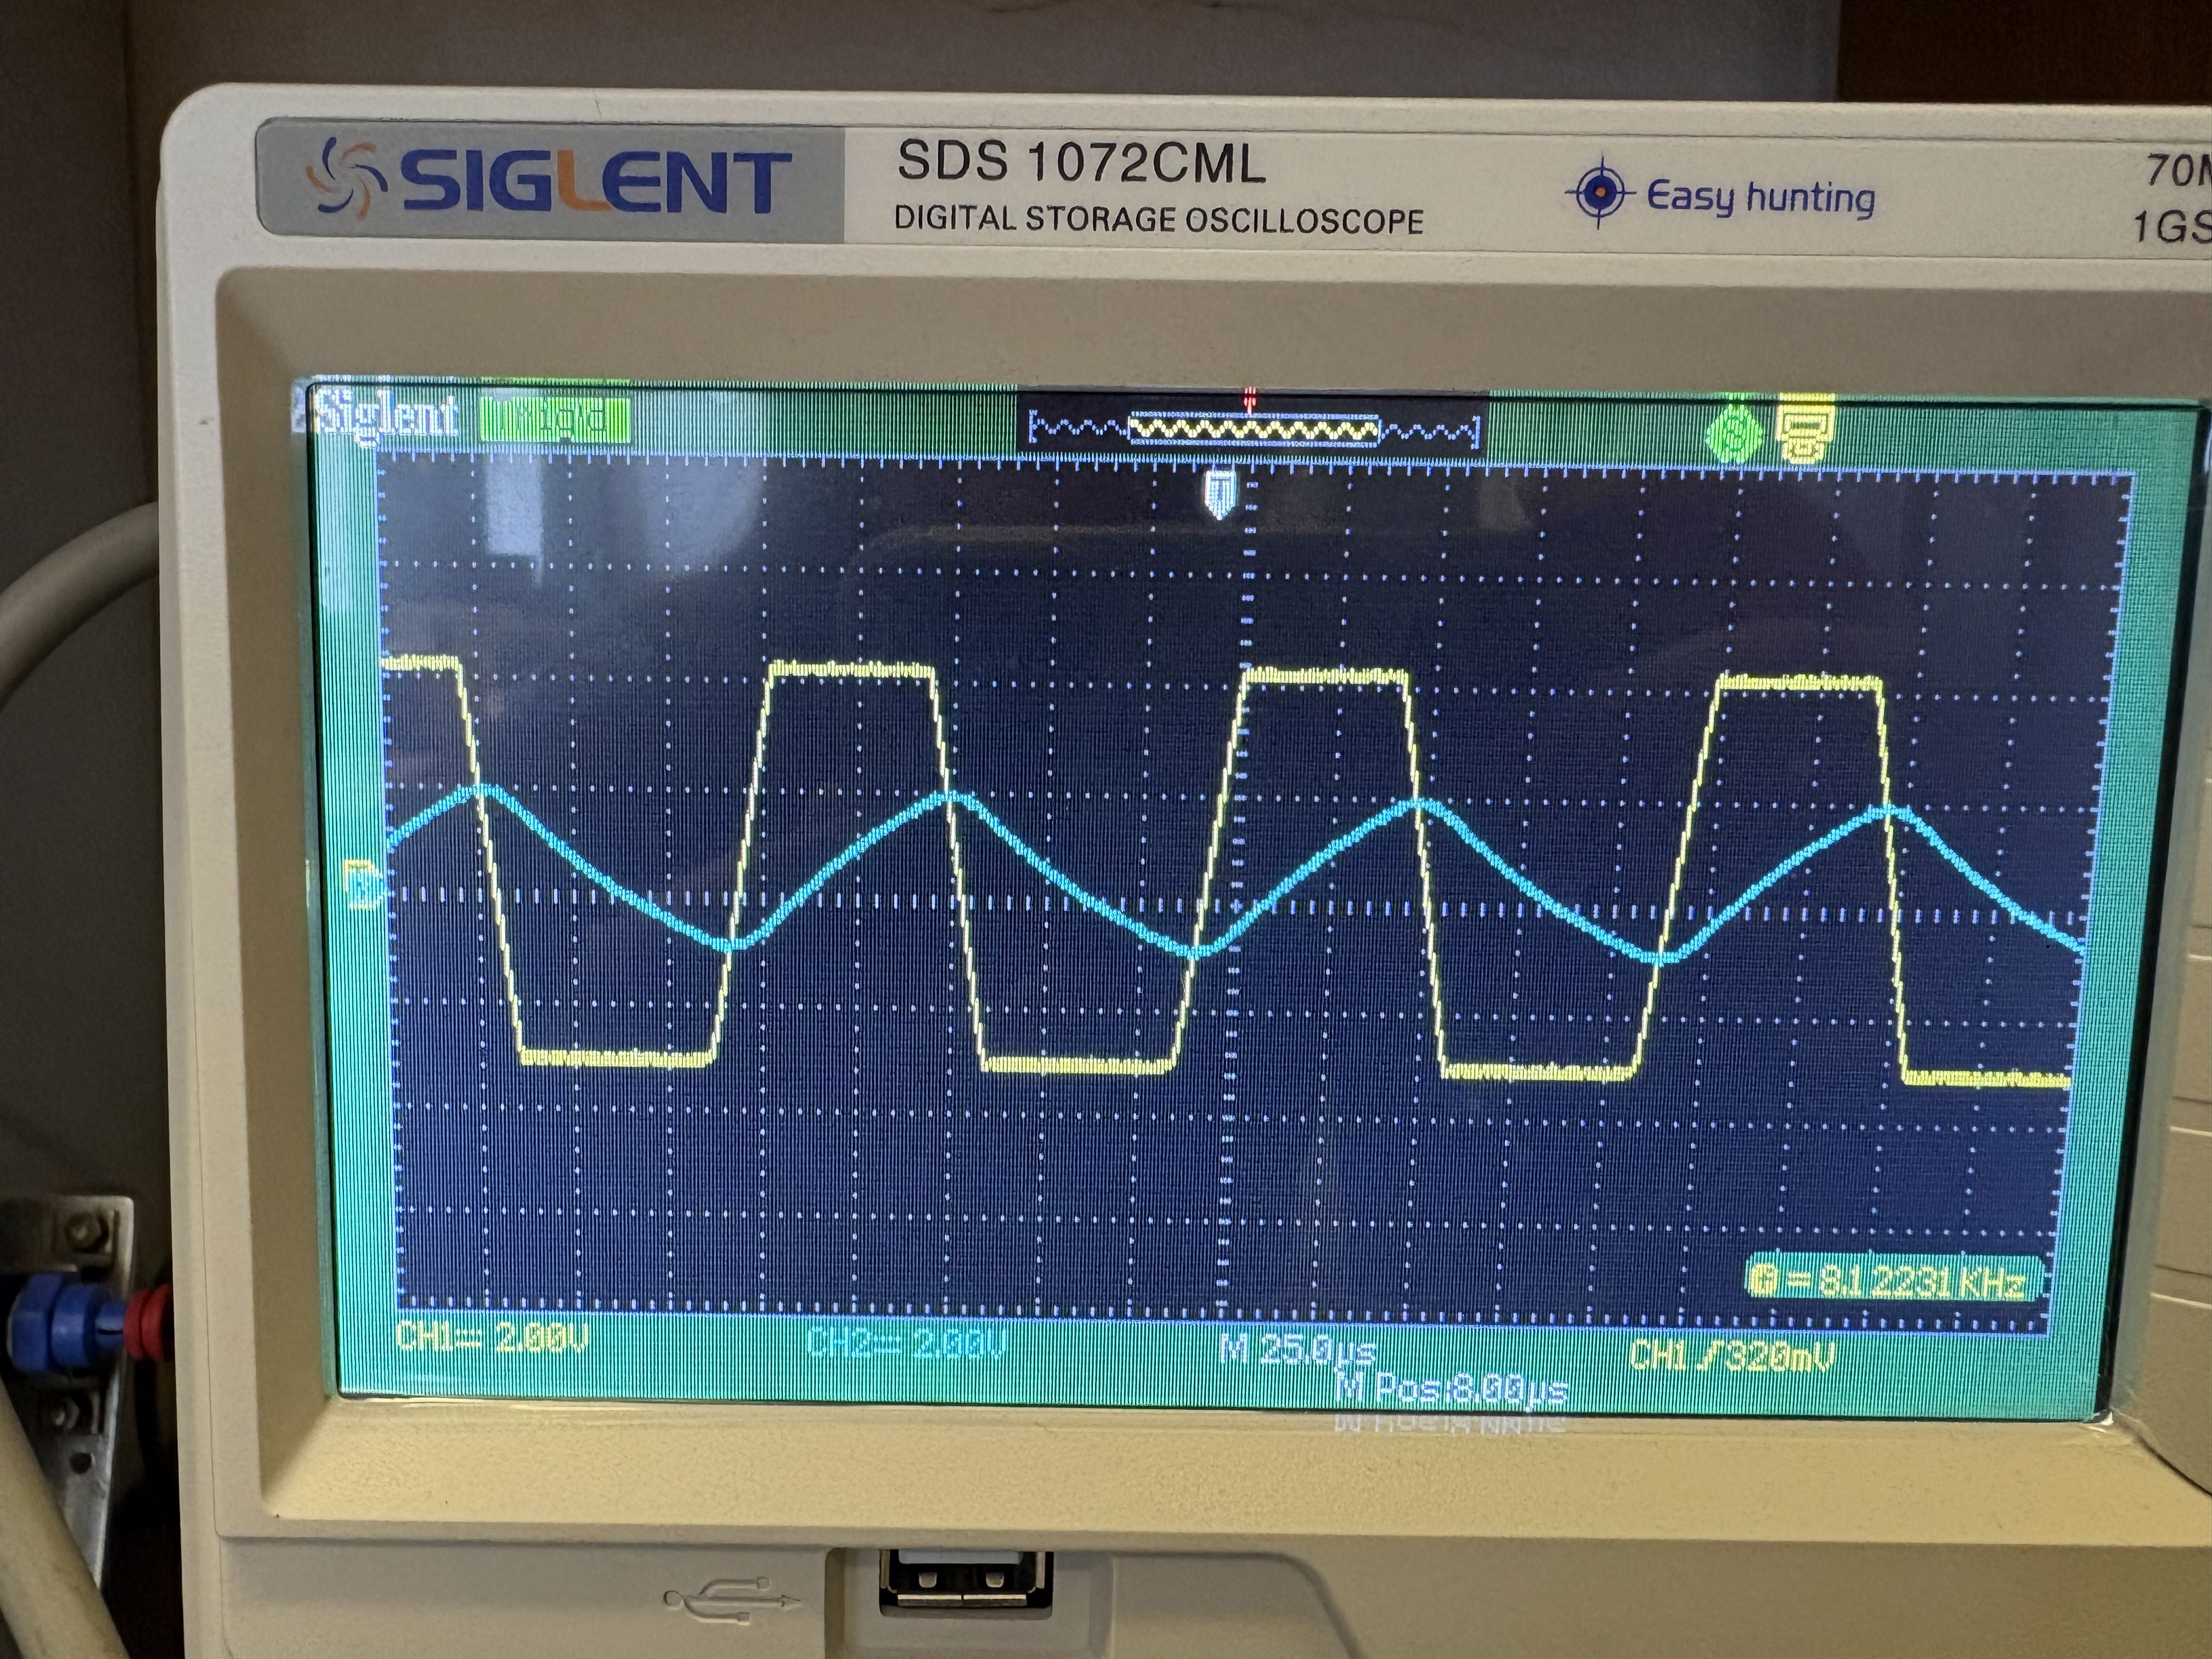
\includegraphics[width=\linewidth]{U2_Uo_AU.jpg}
        \caption{AU: Measurement of U$_{2}$ on channel 2 and U$_{out}$ on channel 1}
    \end{subfigure}

    \caption{Different measured waveforms of the relaxation 
    oscillator setup with two operational amiplifiers, TL071CP 
    and $\mu$A741CN; displaying inputs and output on the channels.}
    \label{fig:relaxation}
\end{figure}
As seen in Table 1 and Figure 3, U1 and Uo share the same waveform shape with different 
amplitude while U2 has a differing shape. When using TL U1 and Uo have ideal square waveform 
with steep edges showing fast switching, while U2 has an equally ideal triangle form with 
well defined peaks.\\
However, when using AU these shapes get rounded and distorted, the rising regime of the 
triangular waveform of both U1 and Uo are no longer as fast, while the triangle waveform of U2 
turns into a rounded series of crests and troughs.\\
U1 and Uo have a similar shape as they are a result of a purely resistive voltage divider. 
On the other hand, U2 is governed by the RC constant, resulting in a charge and discharge behaviour which 
can be seen in the triangular form of the signal. In the case of the AU opamp, the low slew rate 
(SR = 0.5 V/$\mu$s) of the opamp causes the distortion of the waveforms, as it inhibits the instant 
switching we saw with the TL opamp having a much higher slew rate (SR = 13 V/$\mu$s).

\subsection{Switching thresholds of the transistor Schmitt trigger circuit}

\begin{figure}[H]
    \centering
    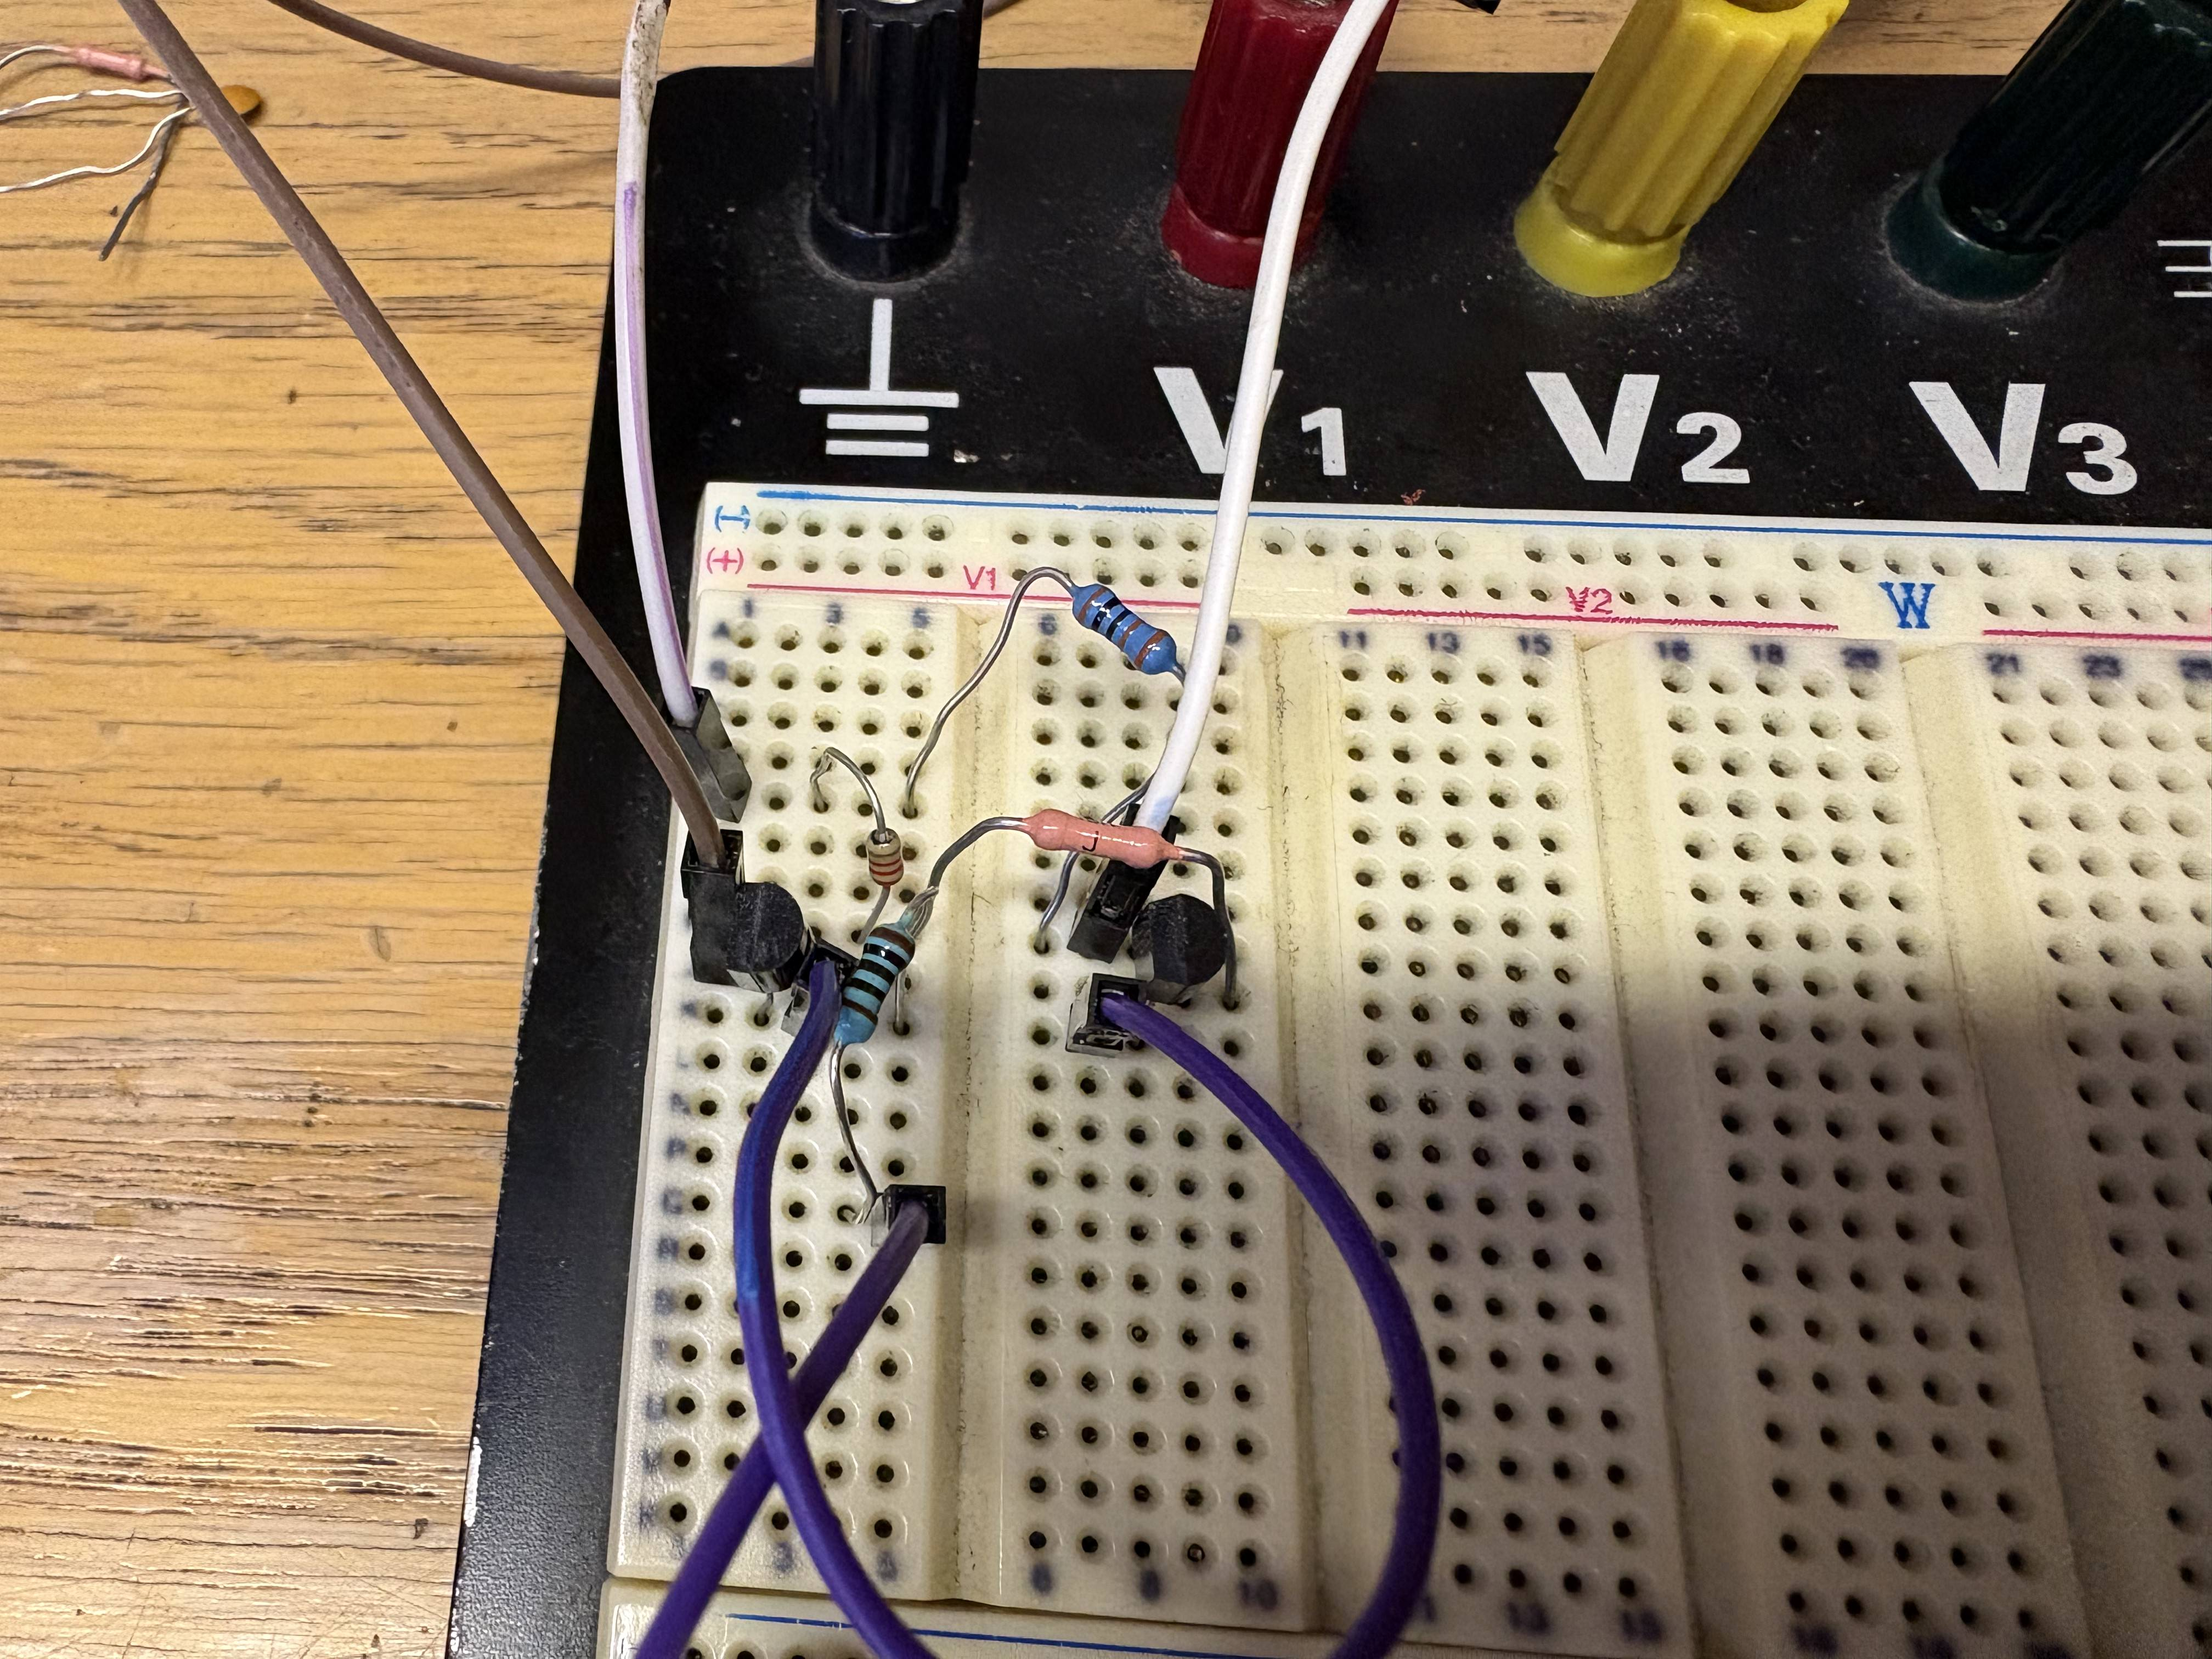
\includegraphics[width=0.5\linewidth]{task4.jpg}
    \caption{Schmitt trigger circuit setup with two transistors and four resistors}
    \label{fig:task4}
\end{figure}

We configured the transistor Schmitt-trigger circuit, and measured the 
input switching thresholds of this configuration. We identified the input 
switching voltages to be around 1.2 - 1.3 V and 0.8 V, where we have 5.004 V and 
0.523 V respectively. Between 0 and 1.2 V we observed a constant 0.523 V, which started 
rising to 0.69 V right before switching at 1.3 V. Similarly, we observed the 5.004 V 
decreasing. Using the following equations, the theoretical switching thresholds are:
\begin{gather*}
    U_{\text{in}\downarrow} = U_{E1} + U_{BE1} \approx 0.21\text{ V} + 0.60\text{ V} \approx 0.81\text{ V}\\[1.2em]
    U_{\text{in}\uparrow} = U_E + U_{BE1} \approx 0.55\text{ V} + 0.65\text{ V} \approx 1.20 \text{ V}
\end{gather*}
These theoretical values align with out measured values near perfectly, with ~1\% deviation error.\\
In the 0 - 1.2 V regime, T1 is off and T2 is on, this results in the output 
voltage being dictated by the saturation collector-emitter voltage of T2. Theoretically, 
the output voltage here is 0.54 V, given by the sum of the voltage drop on the shared 
emitter resistor and the saturation voltage of the collector-emitter on T2. 
Here we measured 0.523 V, giving only 3\% error. As T1 starts to conduct 
the output voltage raises, this is what we measured between 1.2 - 1.3 V right before 
switching, where the output voltage was 0.69 V. \\
In the upper saturation limit, the output voltage should be the full 5 V of the 
positive supply theoretically, as T2 shuts off and T1 is saturated, delivering rail to rail 
output. However, here we measure a value 0.004 V above the positive supply voltage, 
we suspect this to be some inaccuracy of measurement, as it cannot be higher than the 
supply voltage, as energy cannot be created.\\
From these switching thresholds we calculate the experimental hysteresis - using 
the middle value of 1.2 - 1.3 V - to be 1.25 - 0.8 = 0.45 V. From the theoretical 
switching voltages (of 1.2 - 0.81) we get the theoretical hysteresis to be 0.39 V.
Giving us a deviation of near 15\% from the theoretical hysteresis. We believe this 
is also a result of the resolution of our triple supply device, as we were unable to 
set an input more precise than 1.2 or 1.3 V, it is possible that our switching threshold 
was closer to 1.2 V which would have resulted in only ~2\% deviation from the theoretical value.

\section{Conclusion}
In Task 1, testing the simple op-amp comparator revealed a switching threshold 
of 1.6 V (close to the theoretical 1.56 V) with positive output reaching 
4.468 V and negative output stopping at -3.058 V. This asymmetric limit occurs because 
standard op-amps are not rail-to-rail devices, causing internal voltage drops across their 
output transistors instead of reaching the full ±5 V supply rails.\newline
Then, adding a 100 k$\Omega$ feedback resistor in task 2, we built an op-amp Schmitt 
trigger with measured switching thresholds at 1.8 V and 1.3 V, corresponding to output 
saturation levels of -3.086 V and 4.36 V. This created an experimental hysteresis of 0.50 V 
that agreed well with theoretical predictions (1.78 V and 1.14 V), demonstrating how positive 
feedback reduces sensitivity to input noise.\newline
In Task 3, a relaxation oscillator was configured using a 6.8 nF capacitor to produce periodic 
signals governed by an RC charging and discharging cycle. Comparing operational amplifiers 
showed that the high-speed TL071 (slew rate 13 V/$\mu$s) produced ideal square and triangular 
waves, whereas the slower $\mu$A741 (slew rate 0.5 V/$\mu$s) distorted the signals into rounded trapezoids.\newline
Finally, the two-transistor Schmitt trigger produced a low baseline output of 
0.523 V (rising to 0.69 V right before switching) while transistor T1 was off and T2 
was saturated. The circuit switched upwards between 1.2 V and 1.3 V to reach a 5.004 V high 
state and switched back down at 0.8 V, yielding an experimental hysteresis of 0.45 V that closely 
matched the theoretical 1.20 V and 0.81 V bounds.

\nocite{*}
\printbibliography 
\end{document}